\documentclass[a4paper,12pt]{article}
\usepackage{graphicx}
\usepackage{listings}
\usepackage{xcolor}
\usepackage{hyperref} 
\usepackage{caption} 
\usepackage{subcaption}
\usepackage{fancyhdr} 
\usepackage{geometry}
\usepackage{titling}
\usepackage{tocbibind}
\usepackage{float} 
\usepackage{array}
\usepackage{longtable}
\usepackage[dvipsnames]{xcolor}

\geometry{top=3cm, bottom=3cm, left=2.5cm, right=2.5cm}

\begin{document}
\thispagestyle{empty} 

\vspace*{1cm} 

\begin{center}
    {\Huge\textbf {Chess Project}}  
    \vspace{1cm}  

    \begin{figure}[h!]
        \centering
        
\includegraphics[width=0.3\textwidth]{Images/logo.jpg}
    \end{figure}
    
    {\large Session 2023-2027}\\[0.2cm]
    \vspace{0.7cm}
    {\Large\textbf {Submitted By: }}\\[0.6cm]
    {\large {Mohammad Bilal \space\space\space 2023-CS-168}}\\[0.6cm]
    {\Large\textbf {Supervised By: }}\\[0.6cm]
    {\large {Mr. Nazeef Ul Haq }}\\[0.4cm]
    {\large {Mr. Waseem }}\\[0.6cm]
    {\Large\textbf {Course: } CSC-200}\\[1.2cm]
    {\LARGE \textbf{ Department of Computer Science}}\\[0.7cm]
    {\Huge \textbf{University of Engineering and}}\\[0.5cm]
    {\Huge \textbf{Technology, Lahore}}\\[0.5cm]
    \vfill
\end{center}

\thispagestyle{empty} 

% all the contents table, figures and tables must have no text on heder footer 

\renewcommand{\contentsname}{Table of Contents}

\tableofcontents

\newpage

\thispagestyle{empty}

\listoffigures

\newpage

\thispagestyle{empty}

\listoftables

\newpage

\pagestyle{fancy}
\fancyhf{}
\fancyhead[L]{\textbf{Chess Project}}
\fancyfoot[R]{{\thepage}}
\fancyfoot[L]{{MOHAMMAD BILAL}}

\section{Project Overview}

\subsection{Description}
This project is a Chess Game developed using the WPF framework in C\#. It leverages the .NET Framework version v4.8 and provides an engaging platform for both multiplayer and single-player modes. The single-player mode offers three difficulty levels: easy, medium, and hard. Additionally, the game adheres strictly to FIDE rules, includes time controls (1m, 3m, 5m, and 10m), and supports advanced features like Undo functionality, offering a draw, and move validation. 

\subsection{Motivation}
The motivation for creating this project stemmed from two key factors:
\begin{itemize}
    \item A desire to learn and understand the practical use of data structures in building real world projects.
    \item A personal admiration for the game of Chess and an eagerness to develop my own version of it with all the main features and functionalities.
\end{itemize}

\subsection{Objectives}
The objectives of the project include the following.
\begin{itemize}
    \item Demonstrate the use of data structures such as arrays, lists, linked lists, stacks, and graphs in a real-world project.
    \item Design and implement a chess game that adheres to the FIDE rules. Also integrate the correct moves notation.
    \item To integrate both multiplayer and Player vs. Computer modes with varying difficulty levels.
    \item To enhance understanding of WPF and the.NET framework.
\end{itemize}

\subsection{Target Audience}
This project aims to:
\begin{itemize}
    \item Beginners and intermediate programmers who wish to explore the practical application of data structures.
    \item Developers interested in creating games using WPF and the.NET Framework.
    \item People who enjoy both Chess and Coding and looking for some fun side activity to broaden their experiences.
\end{itemize}

\subsection{Features}
\begin{longtable}{|p{0.25\textwidth}|p{0.7\textwidth}|}
    \caption{Game Features}
    \hline
    \textbf{Feature} & \textbf{Description} \\
    \hline
    Multiplayer Mode & Allows two human players to play against each other on a same device. \\
    \hline
    Notation & Proper Display of Moves Notation (according to FIDE rules) for ease of users. \\
    \hline
    Player vs. Computer Mode & Enables a single player to compete against the AI with three difficulty levels: easy, medium, and hard. \\
    \hline
    Time Controls & Provides four time control options: 1 minute, 3 minutes, 5 minutes, and 10 minutes. \\
    \hline
    FIDE-Compliant Rules & Adheres to official Chess rules, including castling, en passant, and pawn promotion. \\
    \hline
    Undo Functionality & Allows players to undo their last move. \\
    \hline
    Offer Draw & Players can offer a draw during the game and if the other player accepts the offer the game results in a draw. \\
    \hline
    Resign & Players can resign during the game if they don't want to continue. \\
    \hline
\end{longtable}

\subsection{Operational Details}
\begin{longtable}{|p{0.25\textwidth}|p{0.7\textwidth}|}
    \caption{Technology Stack}
    \hline
    Framework & .NET Framework v4.8. \\
    \hline
    UI Framework & WPF (Windows Presentation Foundation)   \\
    \hline
    Language & C\# \\
    \hline
    IDE & Visual Studio 2022 Community Edition \\
    \hline
    Coding Style & Pascal Case for Class members and methods. Camel Case for local variables. \\
    \hline
\end{longtable}

\section{Use Cases}

\subsection{Landing Page}

\begin{longtable}{|m{0.25\textwidth}|m{0.7\textwidth}|}
    \caption{Landing Page} \\
    \hline
    Name & Landing page \\
    \hline
    Actor & Player \\
    \hline
    Description & It displays the options that the player can explore in this game. \\ 
    \hline
\end{longtable}

\begin{figure}[H]
    \centering
    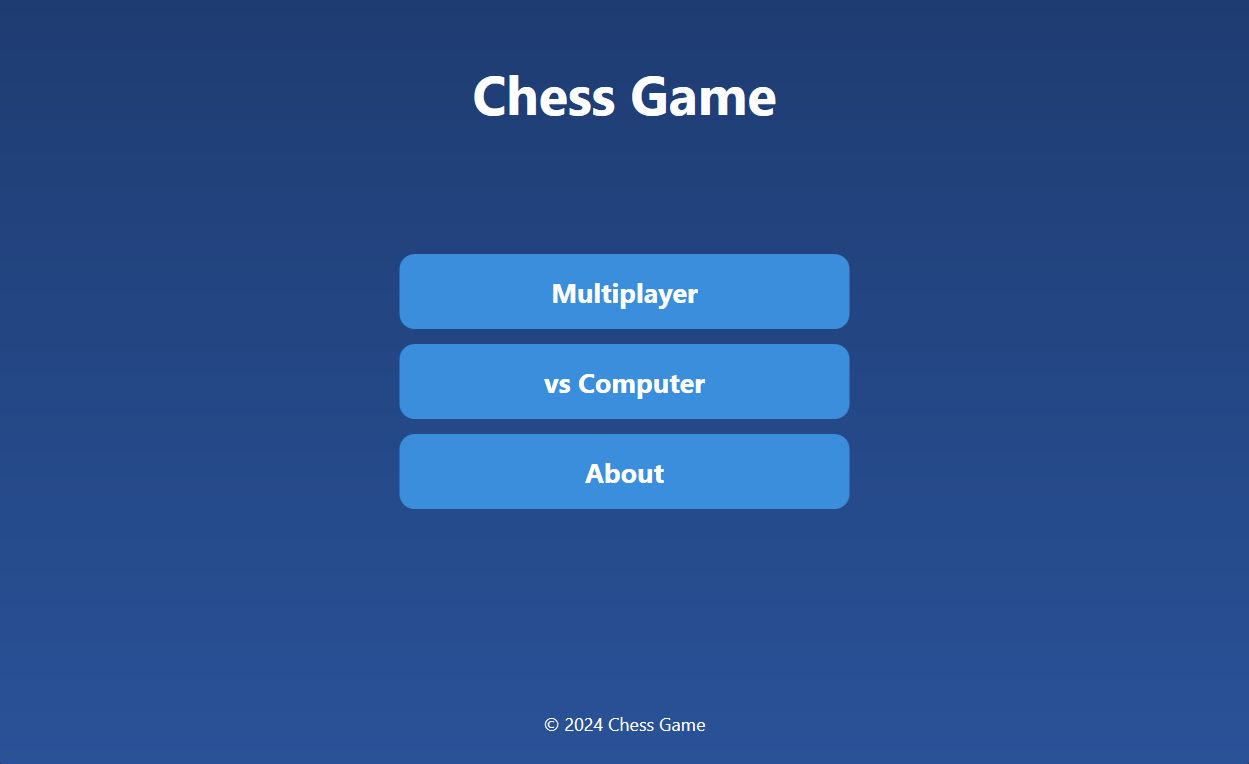
\includegraphics[width=0.7\linewidth]{Images/Use Cases/landingPage.png}
    \caption{Landing Page}
    \label{fig:landingPage}
\end{figure}
    
\subsection{Multi-Player Select Options}

\begin{longtable}{|m{0.25\textwidth}|m{0.7\textwidth}|}
    \caption{Multi-Player Select Options} \\
    \hline
    Name & Multi-player pop-up \\
    \hline
    Actor & Player \\
    \hline
    Description & It displays the time controls and the color that the player can select. \\ 
    \hline
\end{longtable}

\begin{figure}[H]
    \centering
    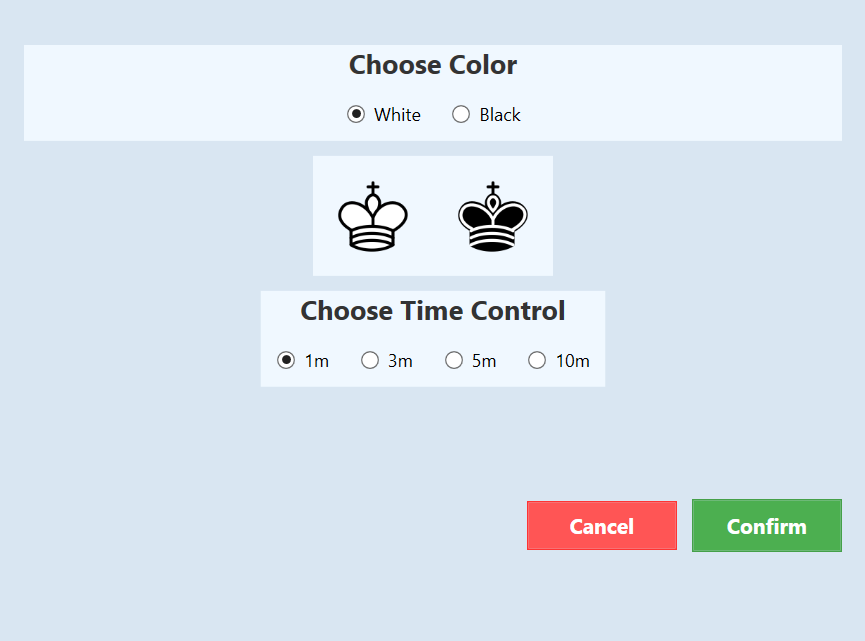
\includegraphics[width=0.7\linewidth]{Images/Use Cases/multiplayerSelectOptions.png}
    \caption{Multi-Player Select 0ptions}
    \label{fig:multiplayerSelectOptions}
\end{figure}

\subsection{Multi-Player Page}

\begin{longtable}{|m{0.25\textwidth}|m{0.7\textwidth}|}
    \caption{Multi-player Page} \\
    \hline
    Name & Game page \\
    \hline
    Actor & Player \\
    \hline
    Description & It is the main page where the game is played. It displays the board, moves, dead pieces and the additional buttons for better experience \\ 
    \hline
\end{longtable}

\begin{figure}[H]
    \centering
    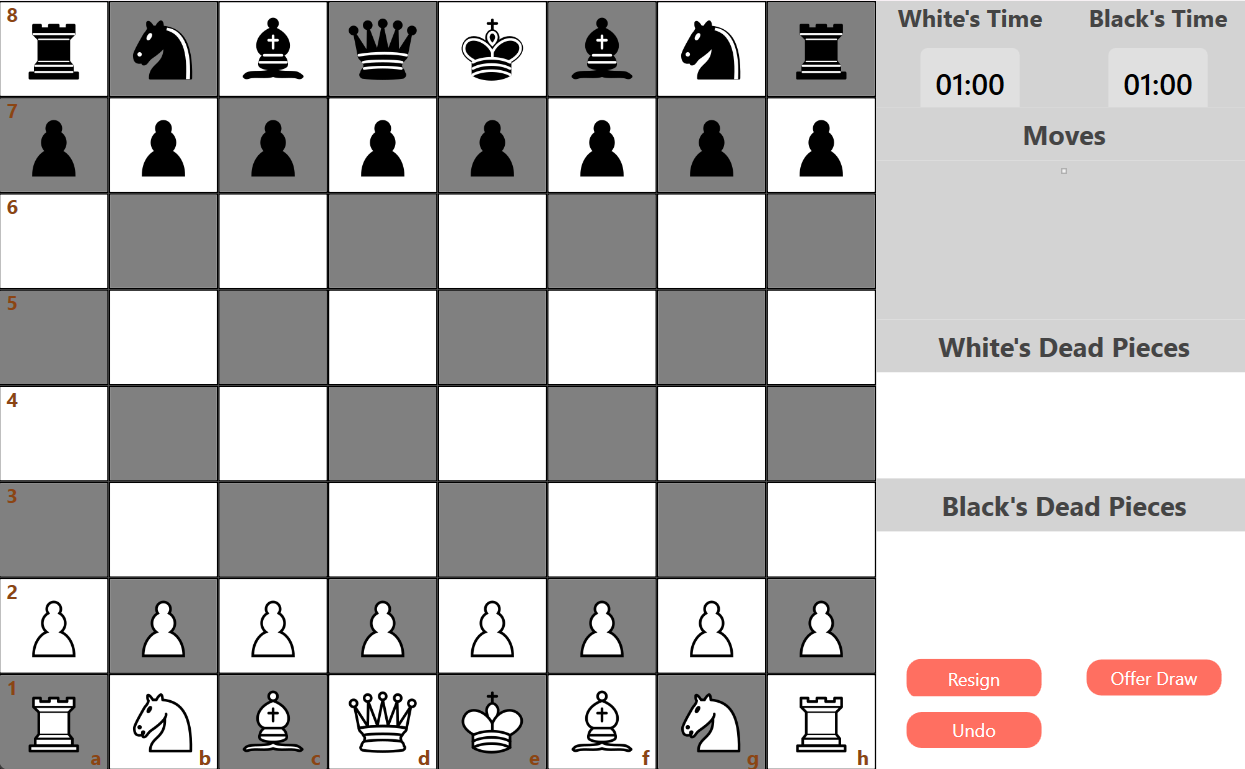
\includegraphics[width=0.7\linewidth]{Images/Use Cases/multiplayerPage.png}
    \caption{Multi-Player Page}
    \label{fig:multiPlayerPage}
\end{figure}
    
\subsection{Promotion Select Options}

\begin{longtable}{|m{0.25\textwidth}|m{0.7\textwidth}|}
    \caption{Promotion Select Options} \\
    \hline
    Name & Promotion selection page \\
    \hline
    Actor & Player \\
    \hline
    Description & It displays the options (Queen, Knight, Bishop and Rook) that your pawn can promote to on reaching enemies last rank.\\ 
    \hline
\end{longtable}

\begin{figure}[H]
    \centering
    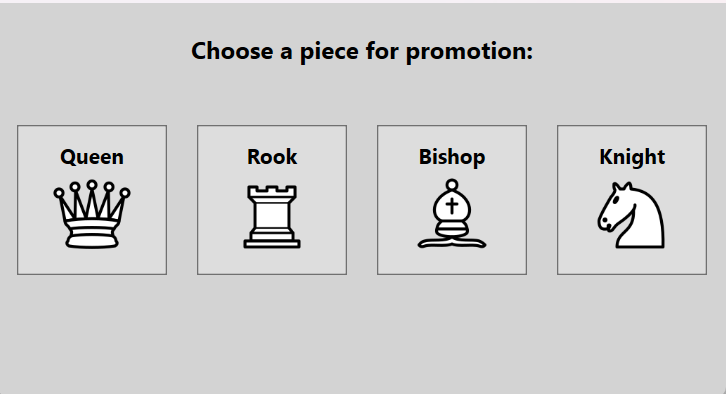
\includegraphics[width=0.7\linewidth]{Images/Use Cases/promotionSelectOptions.png}
    \caption{Promotion Select Options}
    \label{fig:promotionSelectOptions}
\end{figure}
    
\subsection{Multi-Player Game Progress}

\begin{longtable}{|m{0.25\textwidth}|m{0.7\textwidth}|}
    \caption{Multi-Player Game Progress} \\
    \hline
    Name & Game page \\
    \hline
    Actor & Player \\
    \hline
    Description & It displays current progress of the game. On top right side are the moves notations, and below are both player's dead pieces\\ 
    \hline
\end{longtable}

\begin{figure}[H]
    \centering
    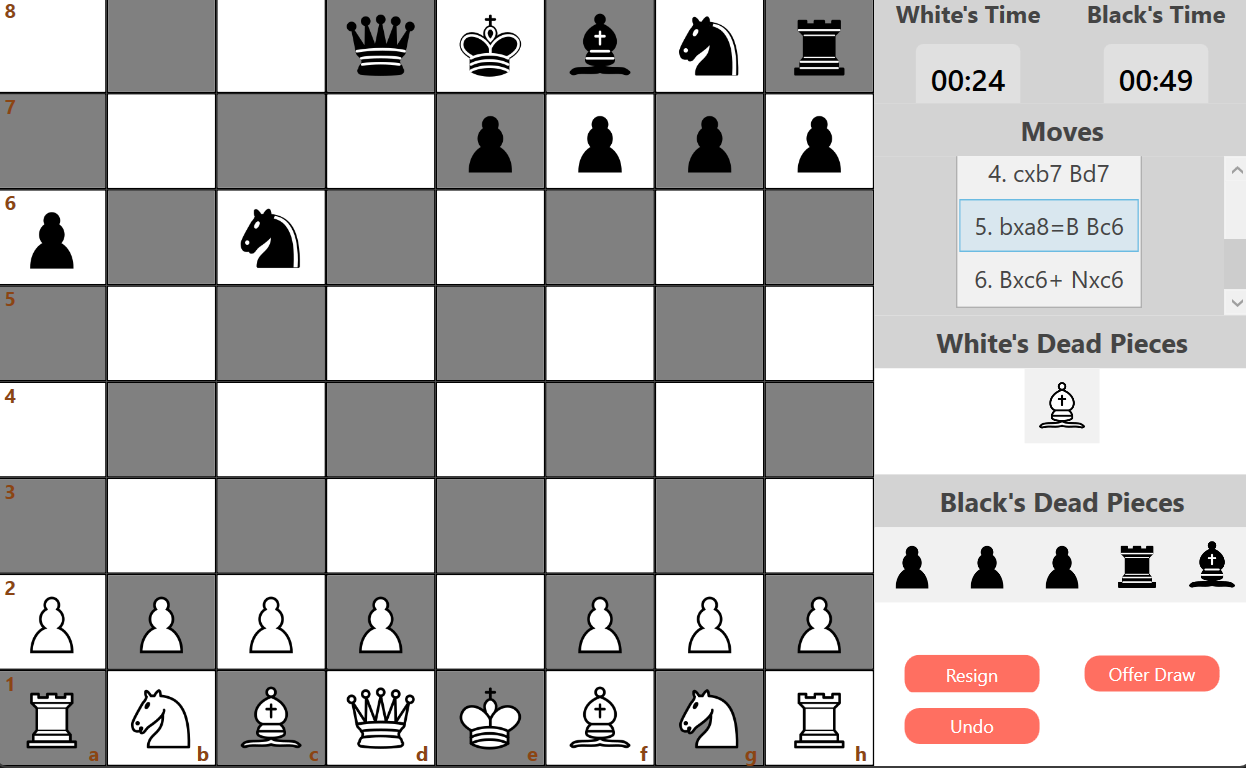
\includegraphics[width=0.7\linewidth]{Images/Use Cases/multiplayerProgress.png}
    \caption{Multi-Player Progress}
    \label{fig:multiplayerProgress}
\end{figure}
    

\subsection{Vs Computer Select Options}

\begin{longtable}{|m{0.25\textwidth}|m{0.7\textwidth}|}
    \caption{Vs Computer Select Options} \\
    \hline
    Name & Vs Computer Select Options \\
    \hline
    Actor & Player \\
    \hline
    Description & It displays the time controls, difficulty levels and the color that the player can select.  \\ 
    \hline
\end{longtable}

\begin{figure}[H]
    \centering
    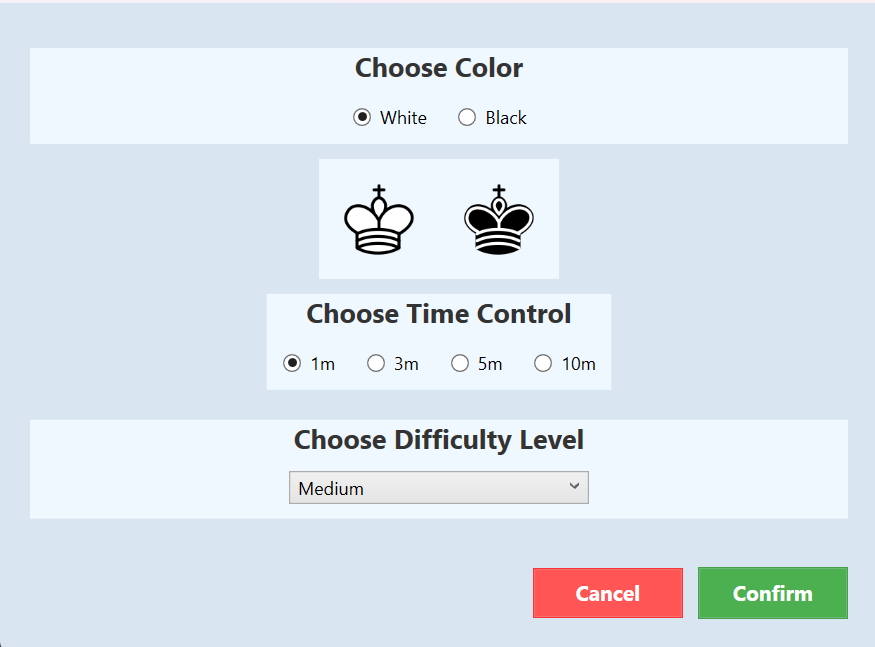
\includegraphics[width=0.7\linewidth]{Images/Use Cases/vsComputerSelectOptions.png}
    \caption{Vs Computer Select Options}
    \label{fig:vsComputerSelectOptions}
\end{figure}
    
\subsection{Vs Computer Progress Page}

\begin{longtable}{|m{0.25\textwidth}|m{0.7\textwidth}|}
    \caption{Vs Computer Progress Page} \\
    \hline
    Name & Vs Computer Progress page \\
    \hline
    Actor & Player \\
    \hline
    Description & It displays current progress of the game. We can clearly see that the time of Black(Computer) is not used at all which shows it's fast move selection. \\ 
    \hline
\end{longtable}

\begin{figure}[H]
    \centering
    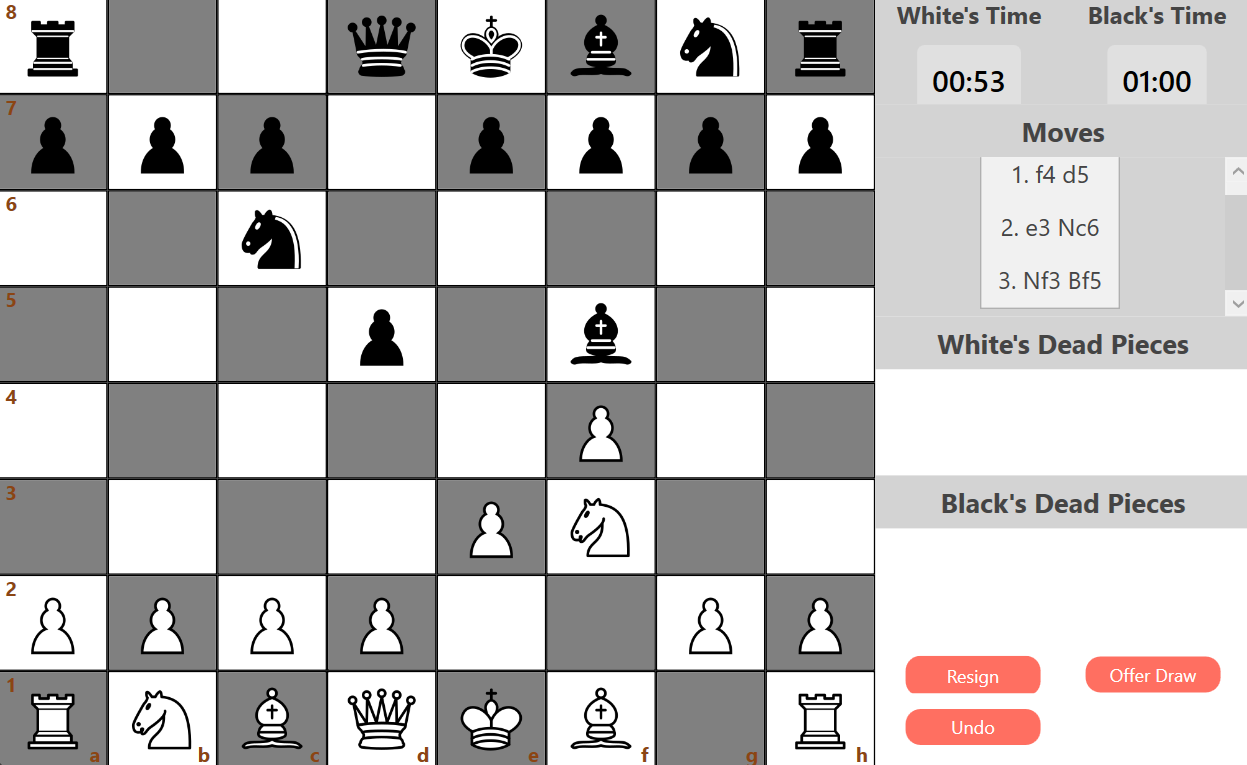
\includegraphics[width=0.7\linewidth]{Images/Use Cases/vsComputerProgress.png}
    \caption{Vs Computer Progress}
    \label{fig:vsComputerProgress}
\end{figure}
    
\subsection{About Page}

\begin{longtable}{|m{0.25\textwidth}|m{0.7\textwidth}|}
    \caption{About Page} \\
    \hline
    Name & About page \\
    \hline
    Actor & Player \\
    \hline
    Description & It displays the developer info, project's features and developer's social links. \\ 
    \hline
\end{longtable}

\begin{figure}[H]
    \centering
    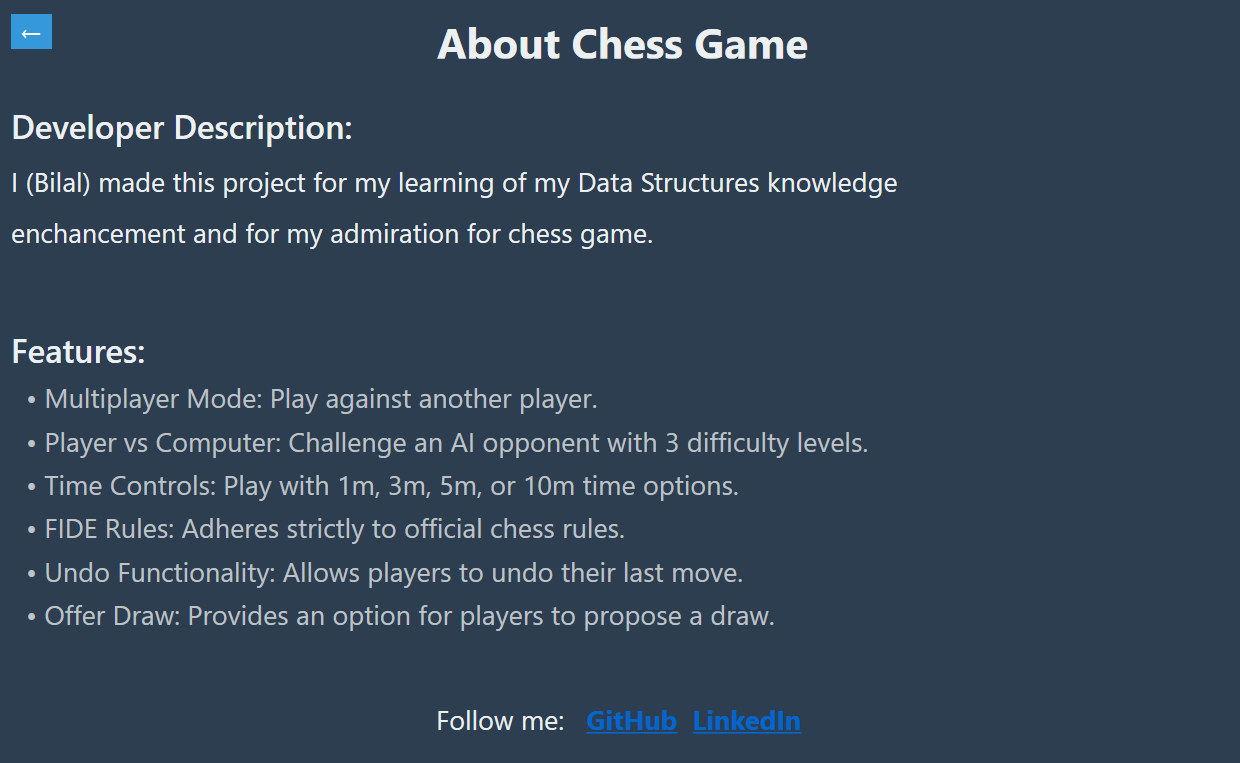
\includegraphics[width=0.7\linewidth]{Images/Use Cases/aboutPage.png}
    \caption{About Page}
    \label{fig:aboutPage}
\end{figure}
    
\section{Test Cases}

\subsection{Test Case 1: Knight Valid Moves}
\textbf{Description}: Ensure that White's Queenside Knight can move to valid squares.\\
\textbf{Expected Outcome}: White's Queenside Knight can move to a3 and c3 from b1.\\
\textbf{Result}: Requirement Satisfied.

\begin{figure}[H]
    \centering
    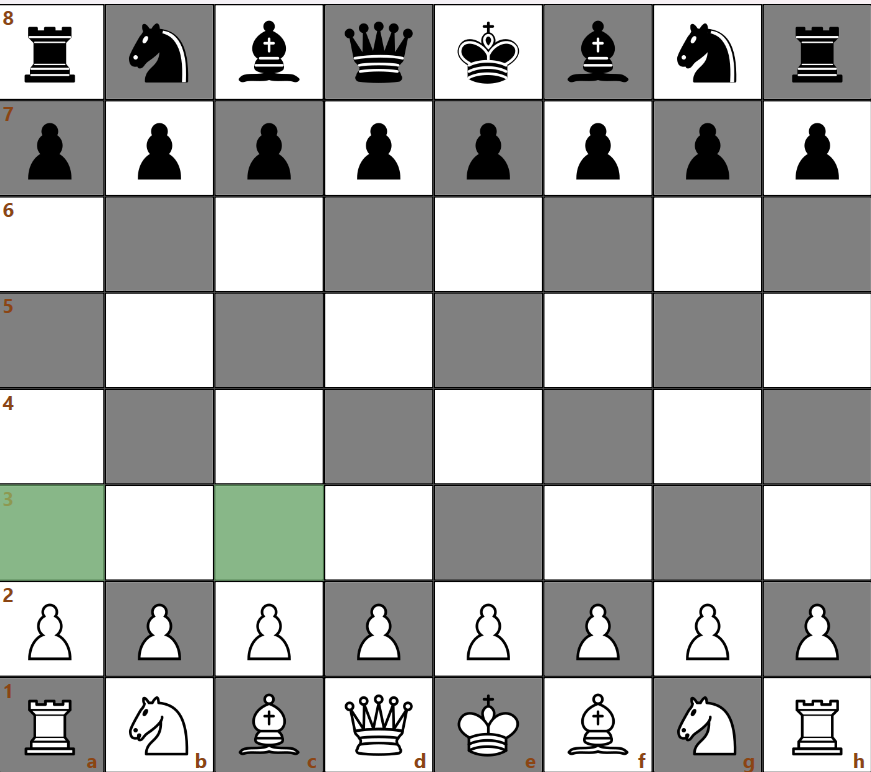
\includegraphics[width=0.6\linewidth]{Images/Test Cases/testCase1Img1.png}
    \caption{On Clicking on the Knight}
    \label{fig:BeforeKnightMove}
\end{figure}

\begin{figure}[H]
    \centering
    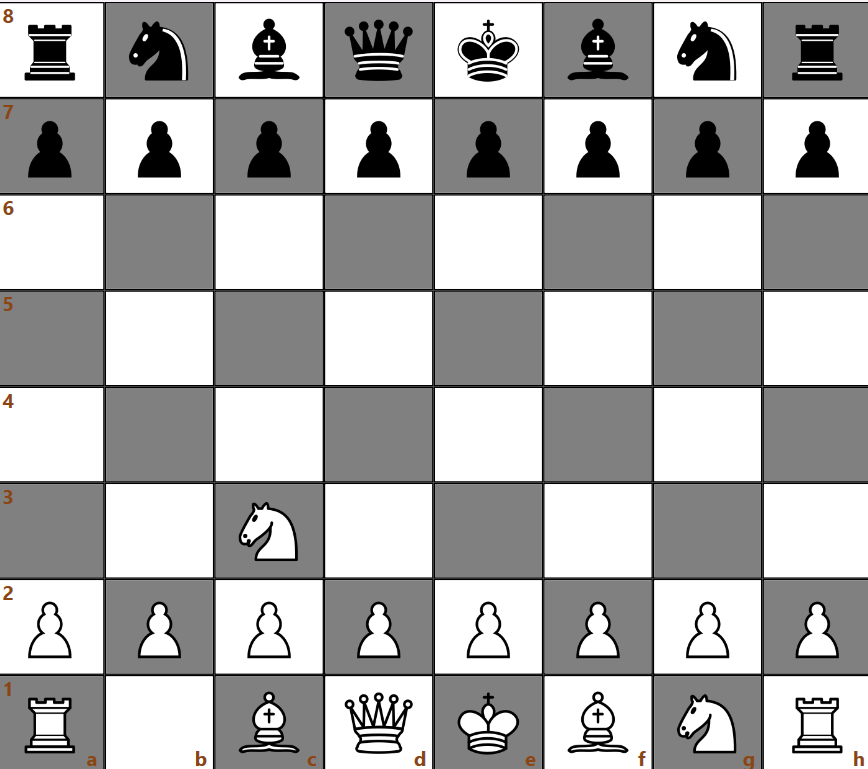
\includegraphics[width=0.6\linewidth]{Images/Test Cases/testCase1Img2.png}
    \caption{On Clicking on the c3 square}
    \label{fig:AfterKnightMove}
\end{figure}

\subsection{Test Case 2: En Passant}
\textbf{Description}: Ensure that Black can perform En Passant capture on White's pawn.\\
\textbf{Expected Outcome}: Black can capture White's pawn on g3 using En Passant.\\
\textbf{Result}: Requirement Satisfied.

\begin{figure}[H]
    \centering
    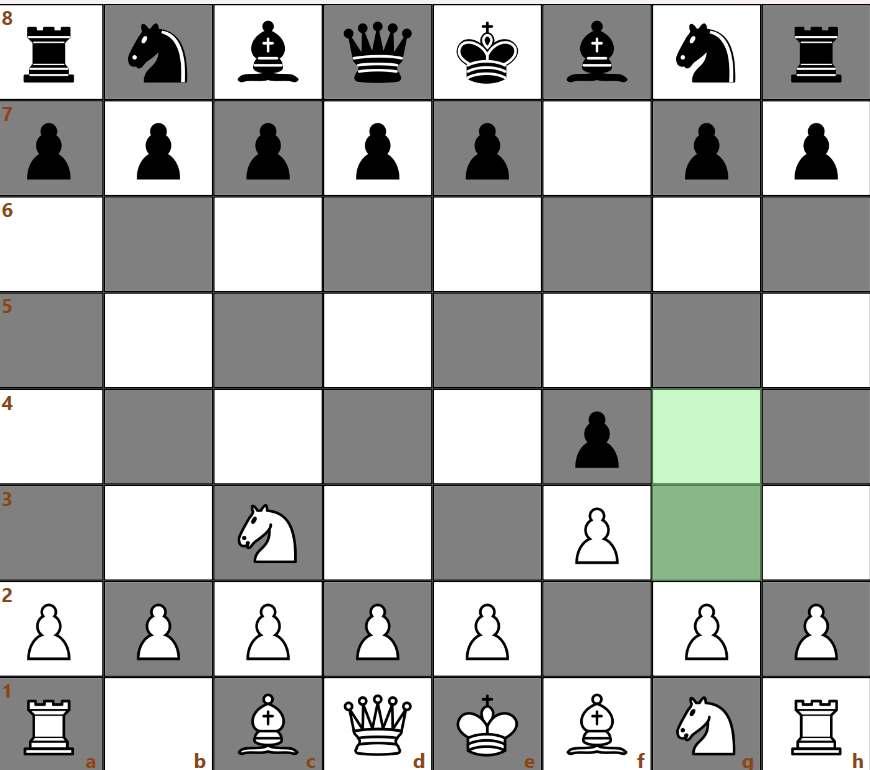
\includegraphics[width=0.6\linewidth]{Images/Test Cases/testCase2Img1.png}
    \caption{Moving White's Pawn}
    \label{fig:WhiteMove}
\end{figure}

\begin{figure}[H]
    \centering
    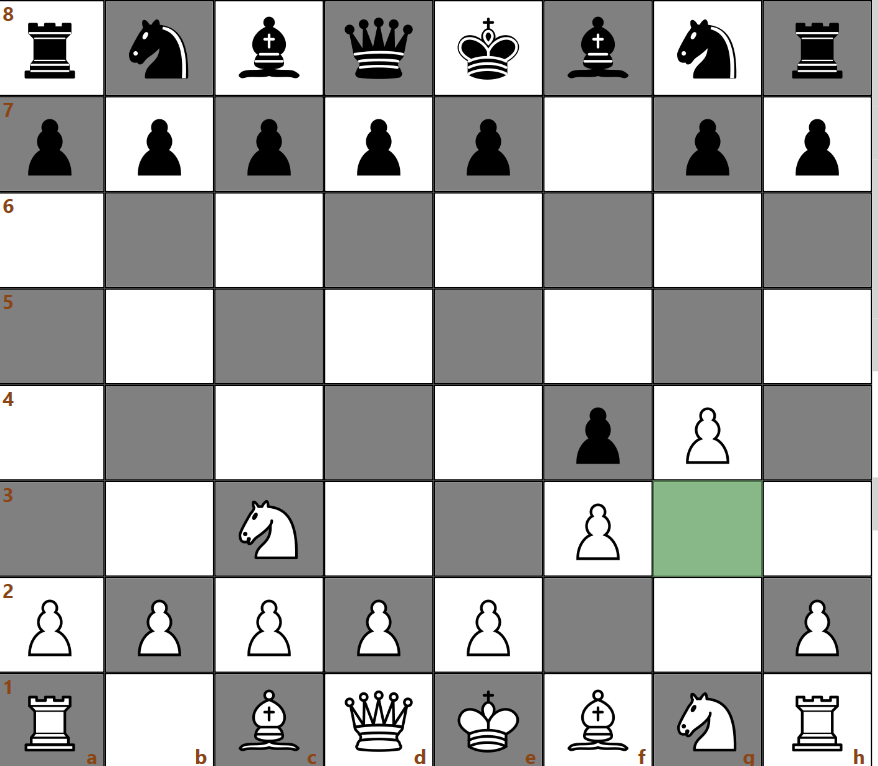
\includegraphics[width=0.6\linewidth]{Images/Test Cases/testCase2Img2.png}
    \caption{Before En Passant Capture}
    \label{fig:BeforeEnPassant}
\end{figure}

\begin{figure}[H]
    \centering
    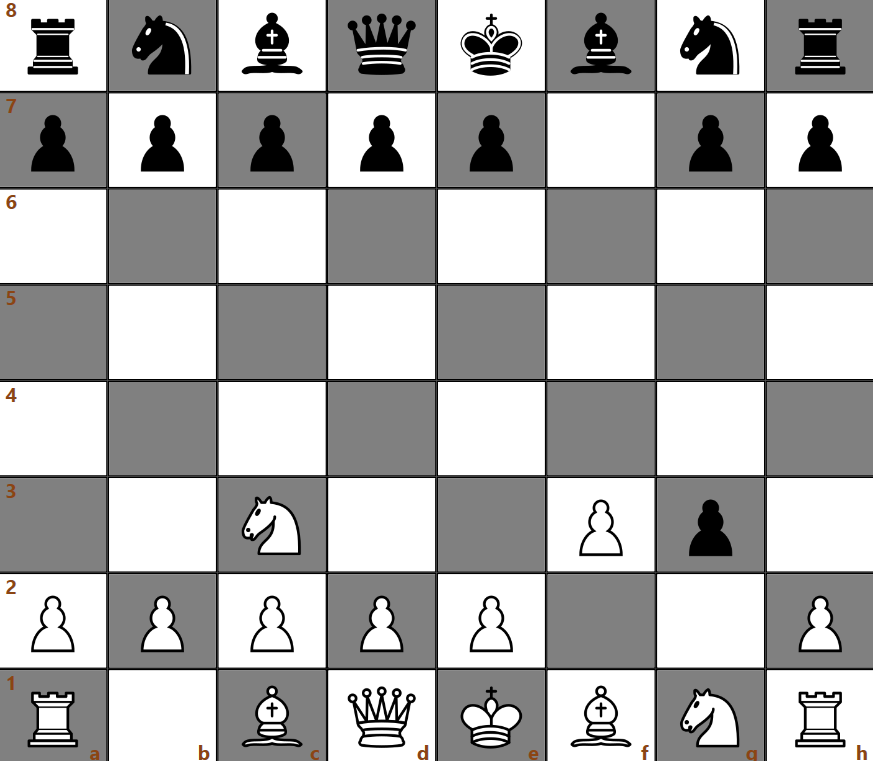
\includegraphics[width=0.6\linewidth]{Images/Test Cases/testCase2Img3.png}
    \caption{After En Passant Capture}
    \label{fig:AfterEnPassant}
\end{figure}

\subsection{Test Case 3: Check}
\textbf{Description}: Ensure that the game detects when a king is in check.\\
\textbf{Expected Outcome}: The game correctly highlights the check condition when the White King is threatened by the Black's Dark-Square Bishop.\\
\textbf{Result}: Requirement Satisfied.

\begin{figure}[H]
    \centering
    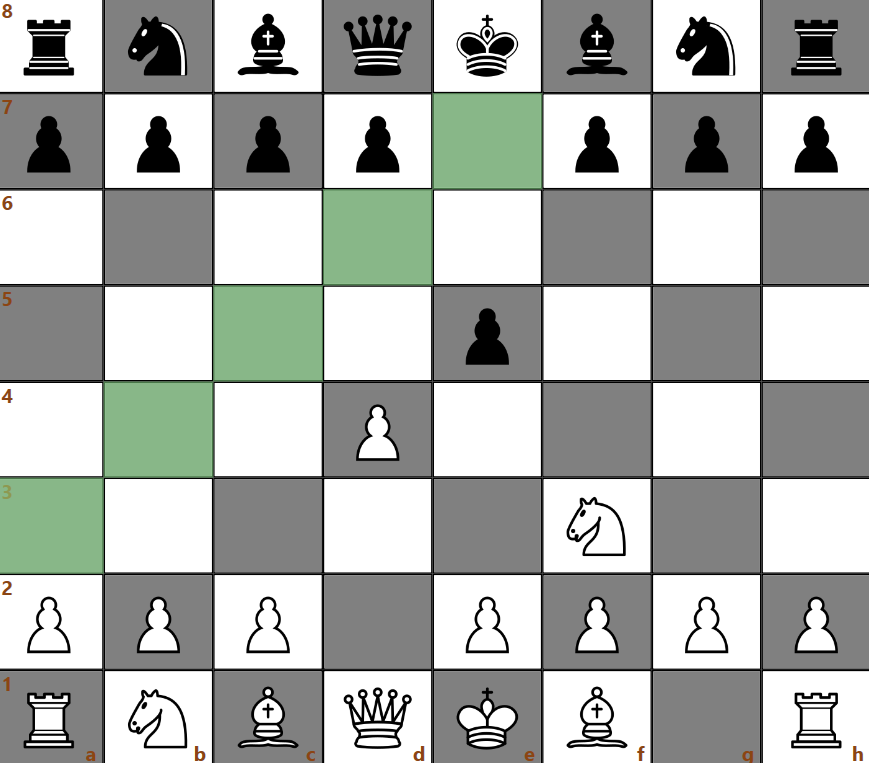
\includegraphics[width=0.6\linewidth]{Images/Test Cases/testCase3Img1.png}
    \caption{Before Check}
    \label{fig:BeforeCheck}
\end{figure}

\begin{figure}[H]
    \centering
    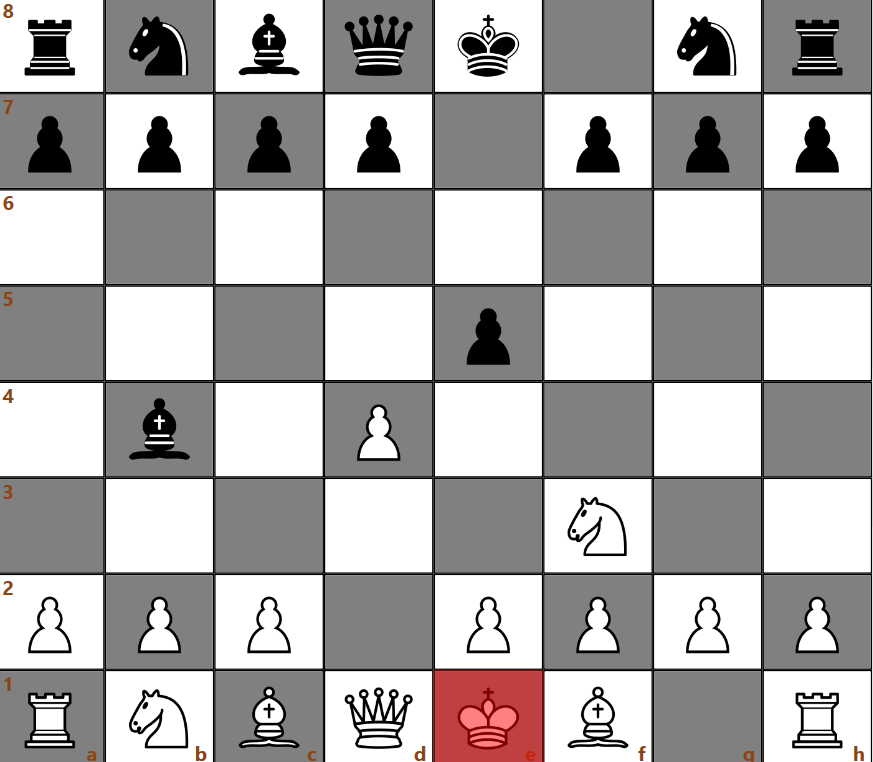
\includegraphics[width=0.6\linewidth]{Images/Test Cases/testCase3Img2.png}
    \caption{After Check}
    \label{fig:AfterCheck}
\end{figure}

\subsection{Test Case 4: En Passant Undo}
\textbf{Description}: Ensure that an En Passant move can be undone correctly.\\
\textbf{Expected Outcome}: En Passant capture can be undone, and the pawn returns to its original position.\\
\textbf{Result}: Requirement Satisfied.

\begin{figure}[H]
    \centering
    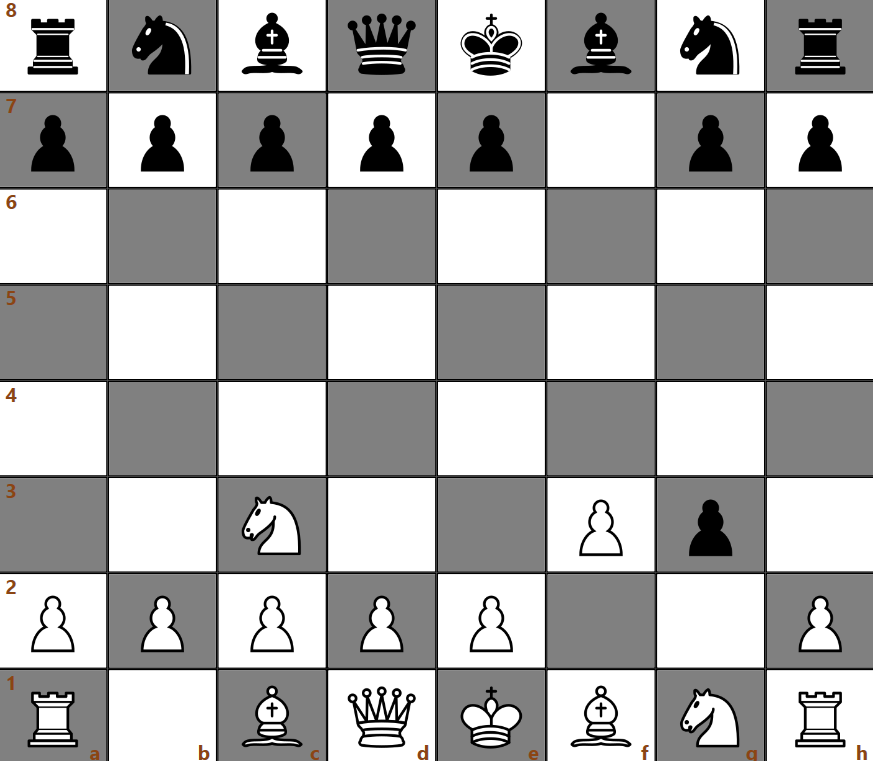
\includegraphics[width=0.6\linewidth]{Images/Test Cases/testCase4Img1.png}
    \caption{Before Undoing En Passant}
    \label{fig:BeforeEnPassantUndo}
\end{figure}

\begin{figure}[H]
    \centering
    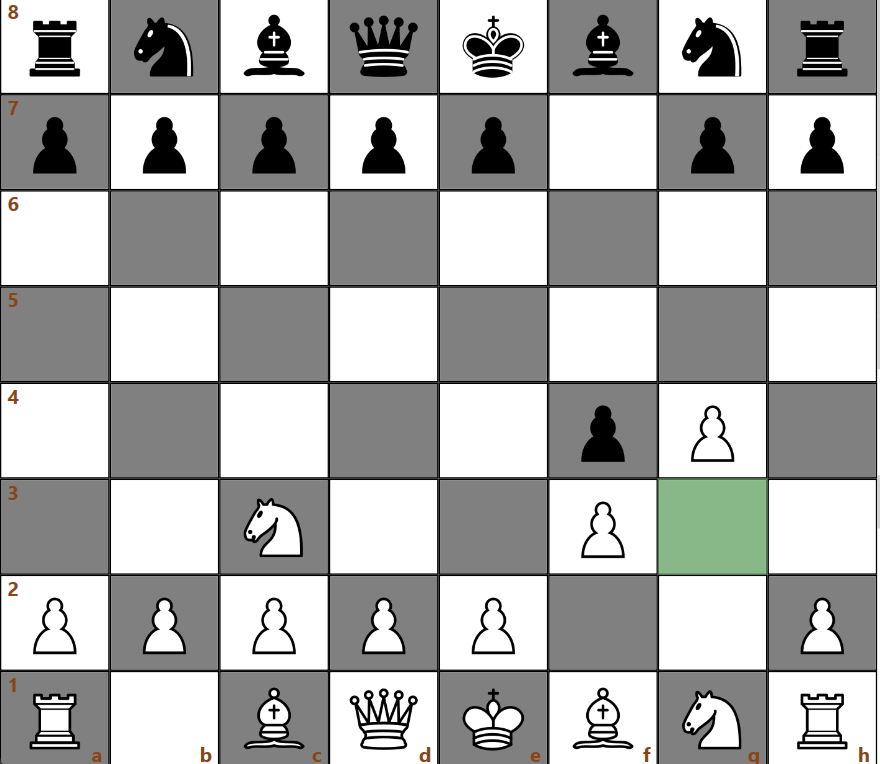
\includegraphics[width=0.6\linewidth]{Images/Test Cases/testCase4Img2.png}
    \caption{After Undoing En Passant}
    \label{fig:AfterEnPassantUndo}
\end{figure}

\subsection{Test Case 5(Part 1): Notation for Promotion}
\textbf{Description}: Ensure that the promotion notation is displayed correctly when a pawn reaches the 8th rank.\\
\textbf{Expected Outcome}: The game displays the correct notation for the promotion of a White pawn to a Queen.\\
\textbf{Result}: Requirement Satisfied.

\begin{figure}[H]
    \centering
    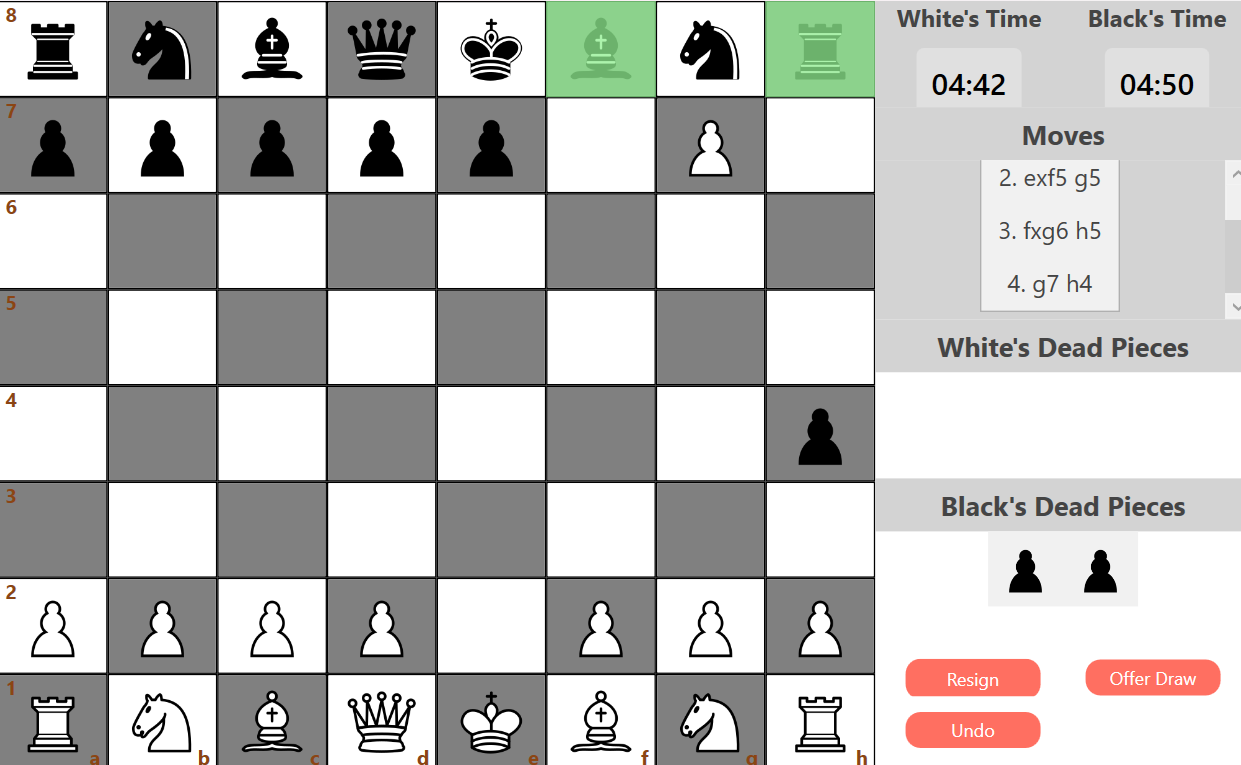
\includegraphics[width=0.7\linewidth]{Images/Test Cases/testCase5Part1Img1.png}
    \caption{Before Promotion Notation}
    \label{fig:BeforePromotionNotation}
\end{figure}

\begin{figure}[H]
    \centering
    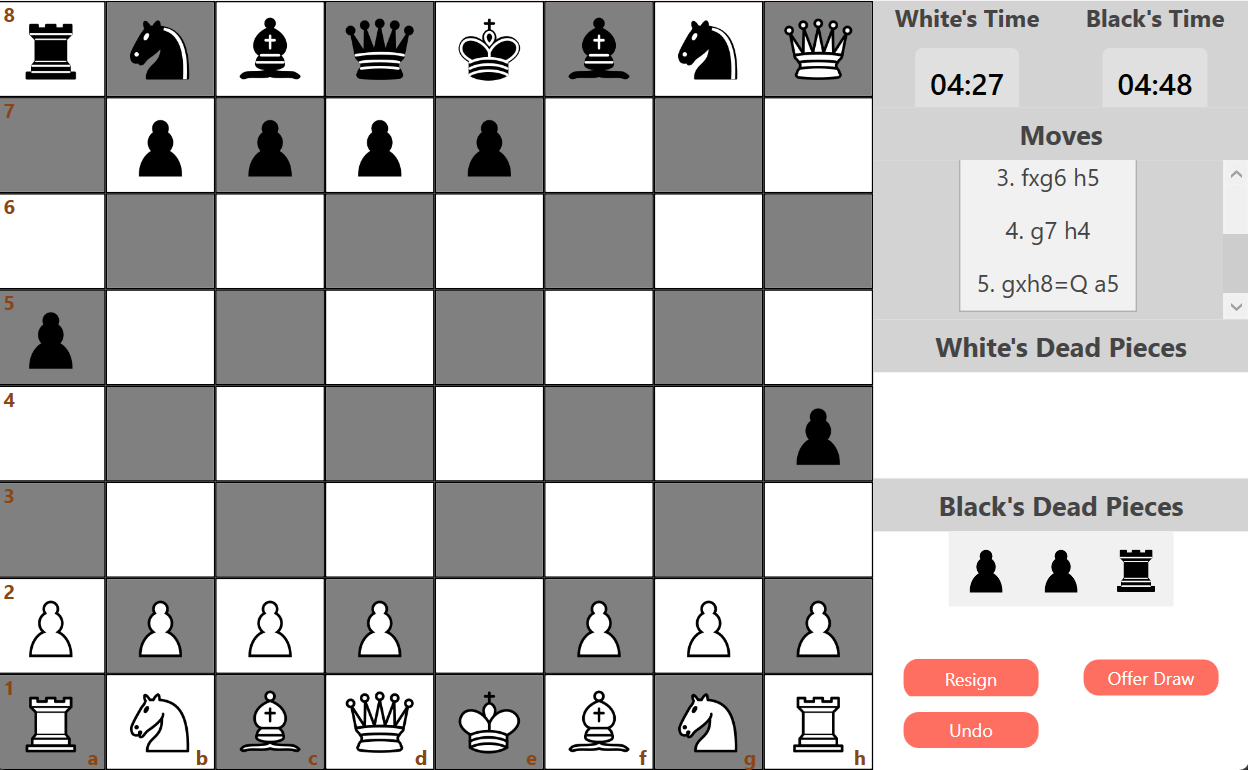
\includegraphics[width=0.7\linewidth]{Images/Test Cases/testCase5Part1Img2.png}
    \caption{After Promotion Notation}
    \label{fig:AfterPromotionNotation}
\end{figure}

\subsection{Test Case 5(Part 2): Notation for Pieces Attacking Same Block}
\textbf{Description}: Ensure that pieces attacking the same block are highlighted correctly.\\
\textbf{Expected Outcome}: The game correctly highlights the squares where multiple pieces are attacking.\\
\textbf{Result}: Requirement Satisfied.

\begin{figure}[H]
    \centering
    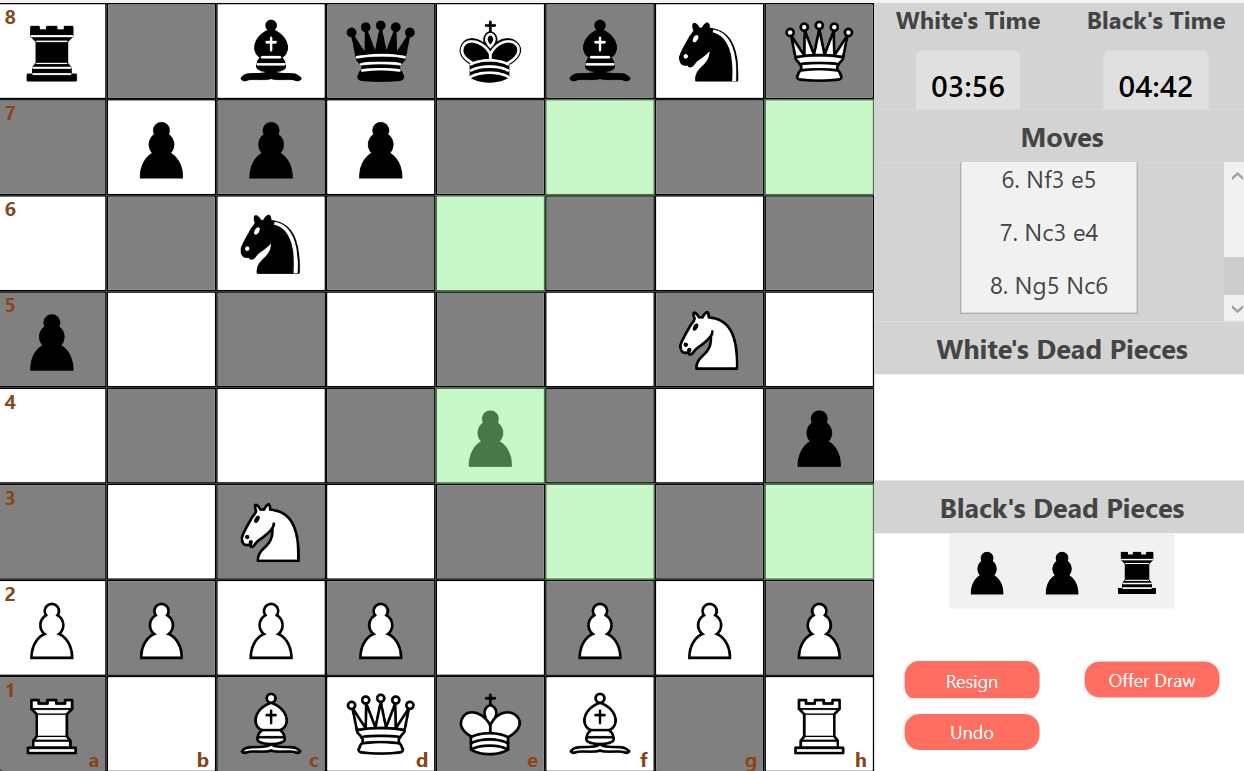
\includegraphics[width=0.7\linewidth]{Images/Test Cases/testCase5Part2Img1.png}
    \caption{Before Pieces Attacking Same Block}
    \label{fig:BeforeAttackingSameBlock}
\end{figure}

\begin{figure}[H]
    \centering
    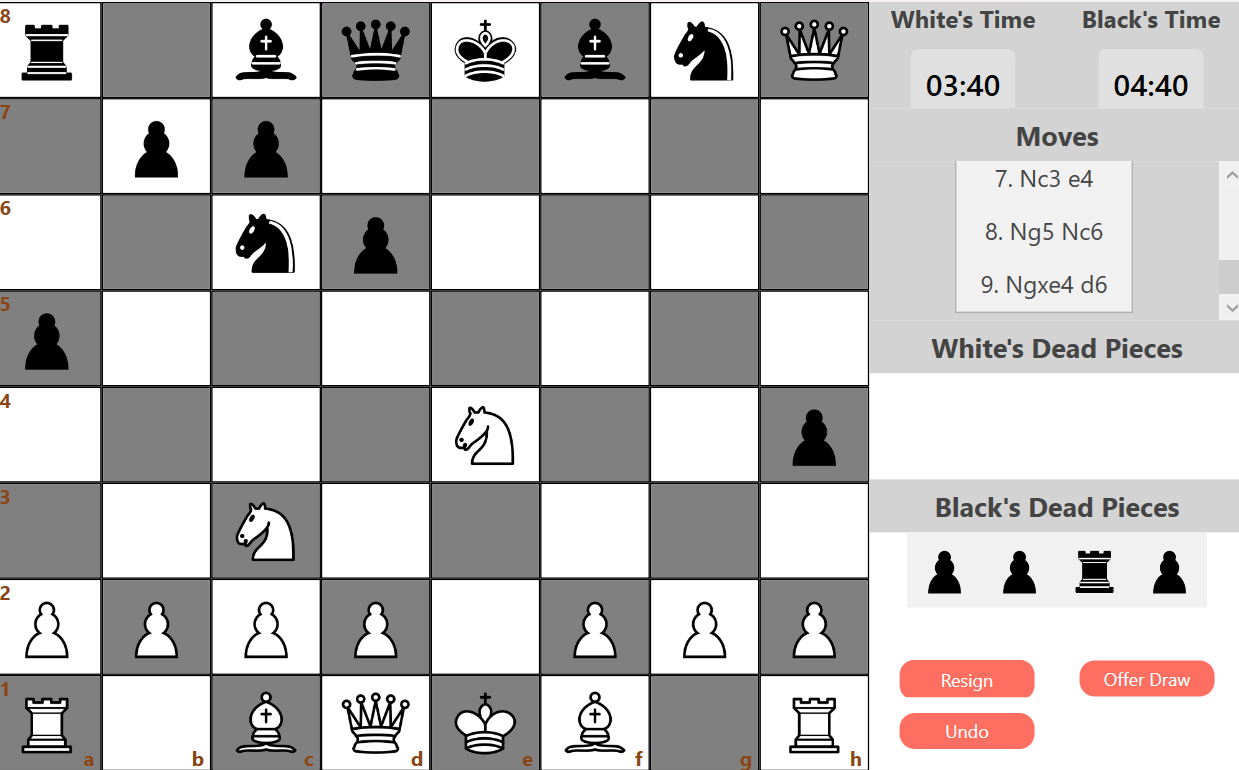
\includegraphics[width=0.7\linewidth]{Images/Test Cases/testCase5Part2Img2.png}
    \caption{After Pieces Attacking Same Block}
    \label{fig:AfterAttackingSameBlock}
\end{figure}

\subsection{Test Case 6: Castling}
\textbf{Description}: Ensure that Black can perform short castle with the king and rook.\\
\textbf{Expected Outcome}: Black can castle by moving the King from e8 to g8 and the Rook from h8 to f8.\\
\textbf{Result}: Requirement Satisfied.

\begin{figure}[H]
    \centering
    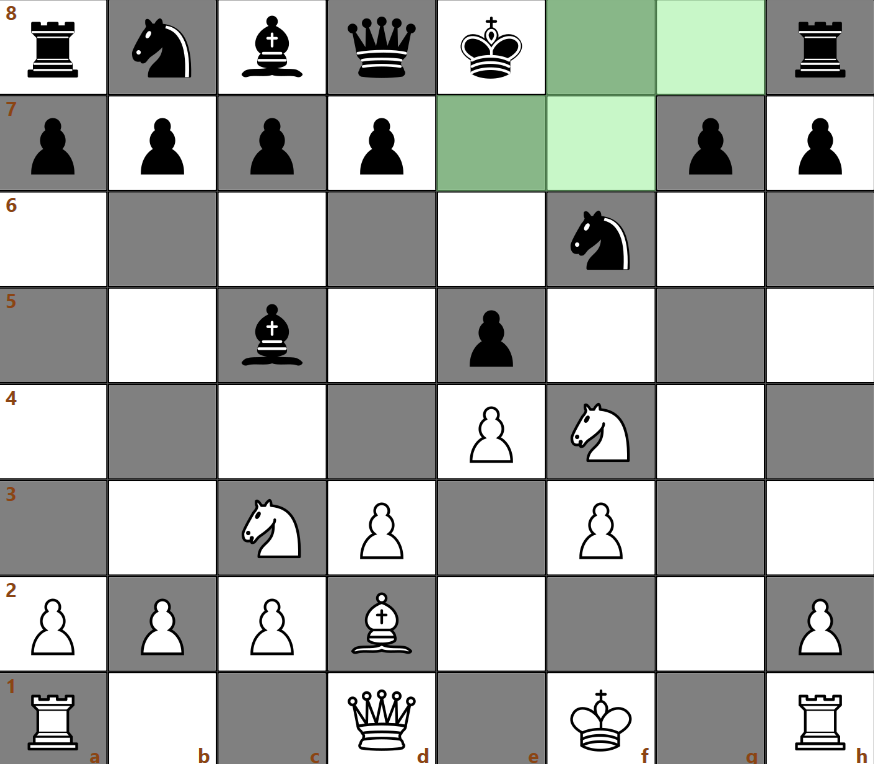
\includegraphics[width=0.6\linewidth]{Images/Test Cases/testCase6Img1.png}
    \caption{Before Castling}
    \label{fig:BeforeCastling}
\end{figure}

\begin{figure}[H]
    \centering
    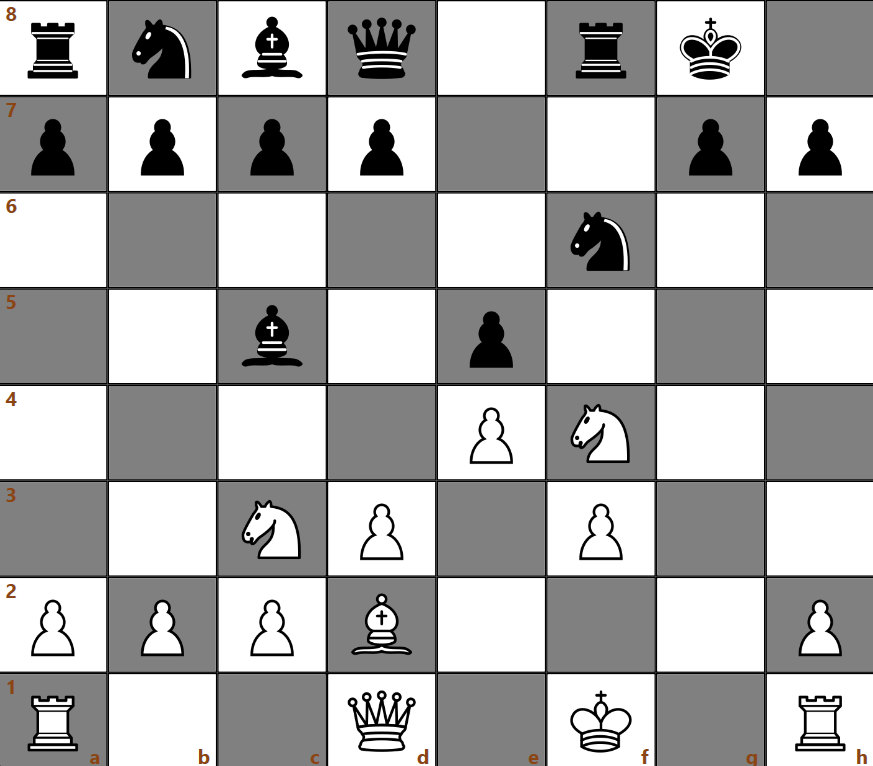
\includegraphics[width=0.6\linewidth]{Images/Test Cases/testCase6Img2.png}
    \caption{After Castling}
    \label{fig:AfterCastling}
\end{figure}

\subsection{Test Case 7: Scholar's Mate}
\textbf{Description}: Ensure that Scholar's Mate can be achieved by White in 4 moves.\\
\textbf{Expected Outcome}: White delivers Scholar's Mate by moving the Queen to f3 and checkmates the Black King.\\
\textbf{Result}: Requirement Satisfied.

\begin{figure}[H]
    \centering
    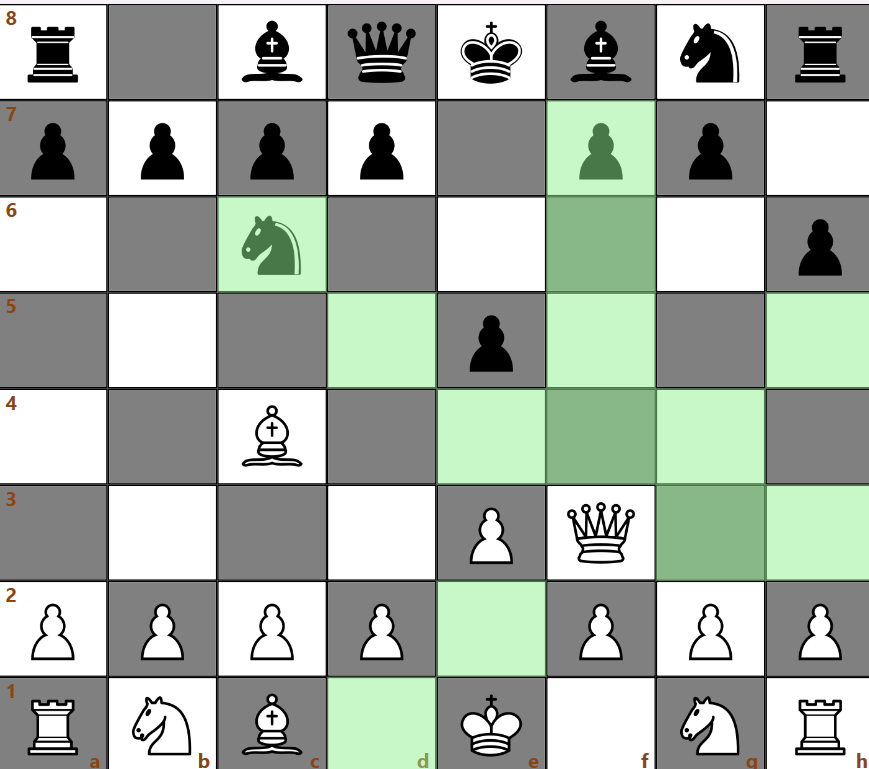
\includegraphics[width=0.6\linewidth]{Images/Test Cases/testCase7Img1.png}
    \caption{Before Scholar's Mate}
    \label{fig:BeforeScholarsMate}
\end{figure}

\begin{figure}[H]
    \centering
    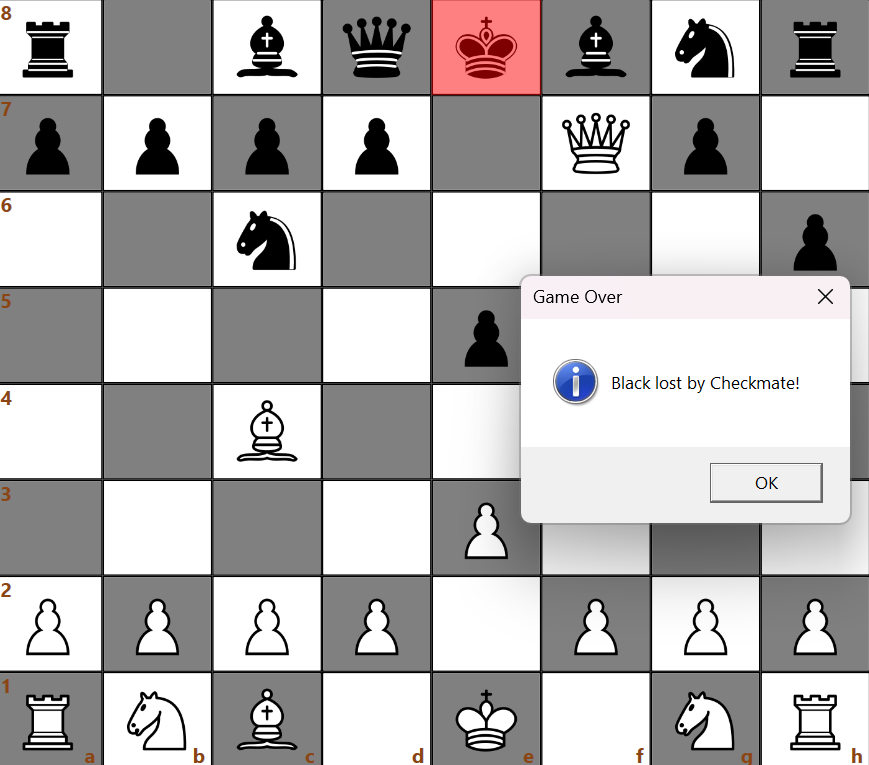
\includegraphics[width=0.6\linewidth]{Images/Test Cases/testCase7Img2.png}
    \caption{After Scholar's Mate}
    \label{fig:AfterScholarsMate}
\end{figure}

\subsection{Test Case 8: Check by Castling}
\textbf{Description}: Ensure that Check by castling is possible.\\
\textbf{Expected Outcome}: The game detects that castling for an open d file leads to check by rook of opponent king.\\
\textbf{Result}: Requirement Satisfied.

\begin{figure}[H]
    \centering
    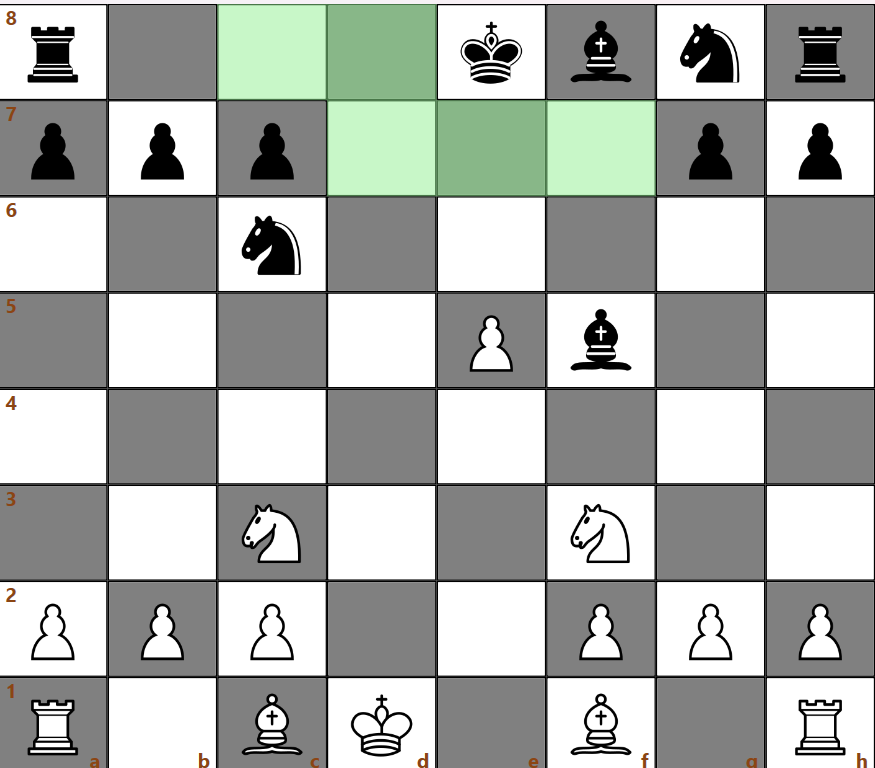
\includegraphics[width=0.6\linewidth]{Images/Test Cases/testCase8Img1.png}
    \caption{Before Check by Castling}
    \label{fig:BeforeCheckByCastling}
\end{figure}

\begin{figure}[H]
    \centering
    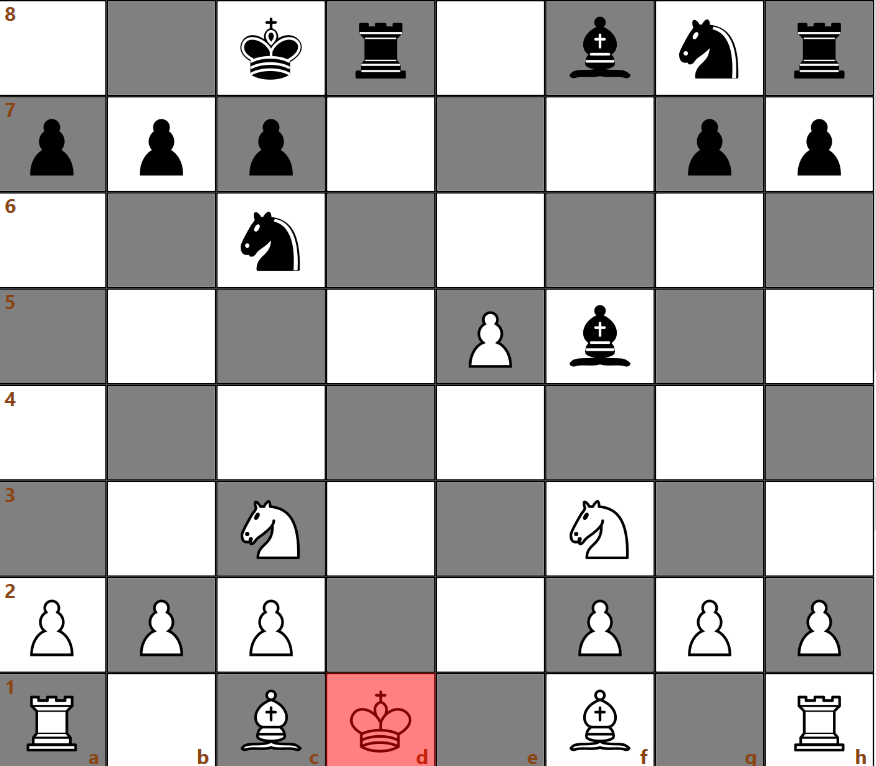
\includegraphics[width=0.6\linewidth]{Images/Test Cases/testCase8Img2.png}
    \caption{After Check by Castling}
    \label{fig:AfterCheckByCastling}
\end{figure}

\subsection{Test Case 9: Promotion Check}
\textbf{Description}: Ensure that a promotion results in check if the opponent's king is in danger.\\
\textbf{Expected Outcome}: The promotion results in check if the opponent's king is in check.\\
\textbf{Result}: Requirement Satisfied.

\begin{figure}[H]
    \centering
    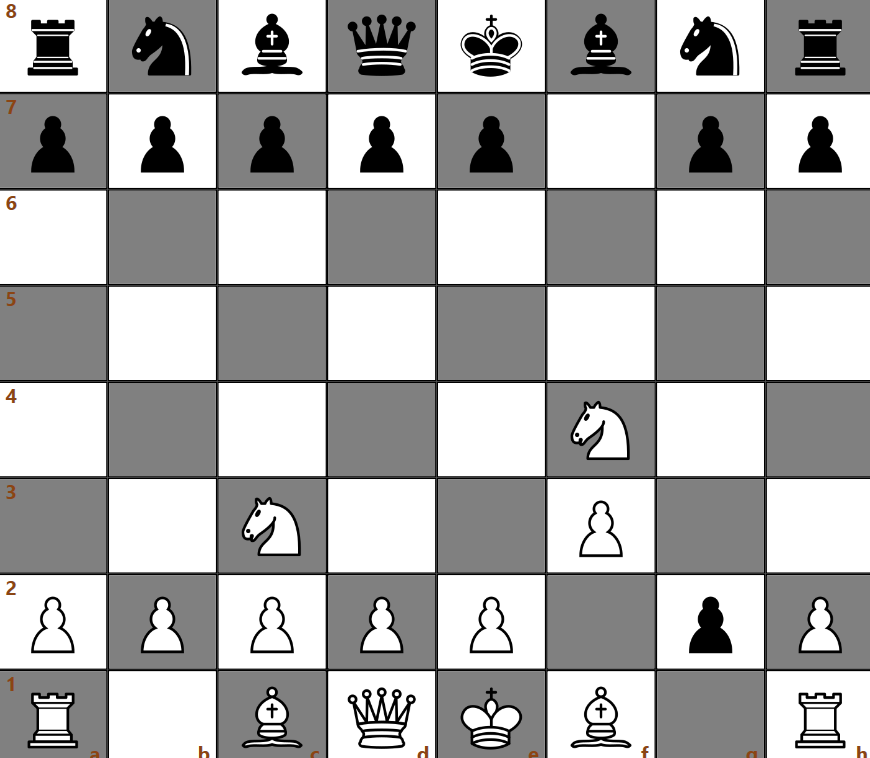
\includegraphics[width=0.6\linewidth]{Images/Test Cases/testCase9Img1.png}
    \caption{Before Promotion Check}
    \label{fig:BeforePromotionCheck}
\end{figure}

\begin{figure}[H]
    \centering
    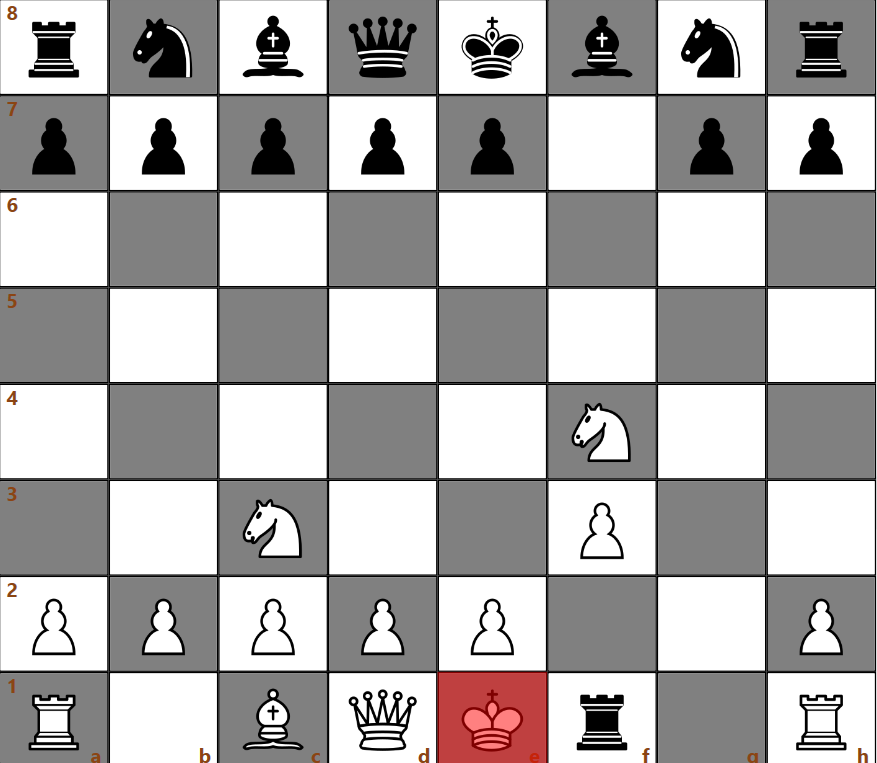
\includegraphics[width=0.6\linewidth]{Images/Test Cases/testCase9Img2.png}
    \caption{After Promotion Check}
    \label{fig:AfterPromotionCheck}
\end{figure}

\subsection{Test Case 10: Computer Move}
\textbf{Description}: Ensure that the computer makes a valid move according to the chosen difficulty.\\
\textbf{Expected Outcome}: The computer makes a valid move on the board for each difficulty level.\\
\textbf{Result}: Requirement Satisfied.

\begin{figure}[H]
    \centering
    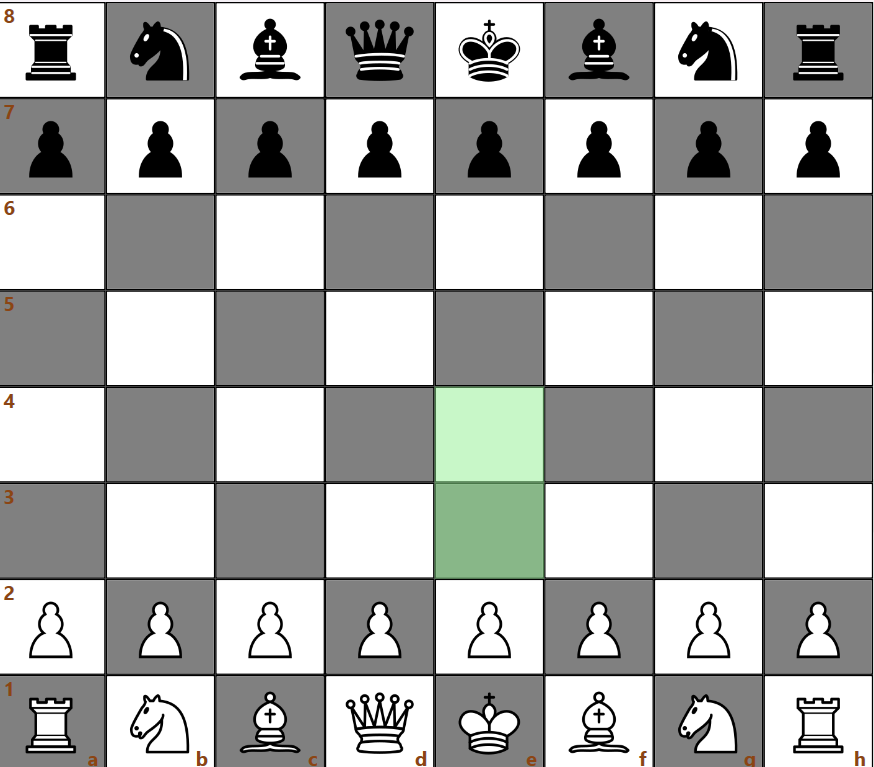
\includegraphics[width=0.6\linewidth]{Images/Test Cases/testCase10Img1.png}
    \caption{Before Computer Move}
    \label{fig:BeforeComputerMove}
\end{figure}

\begin{figure}[H]
    \centering
    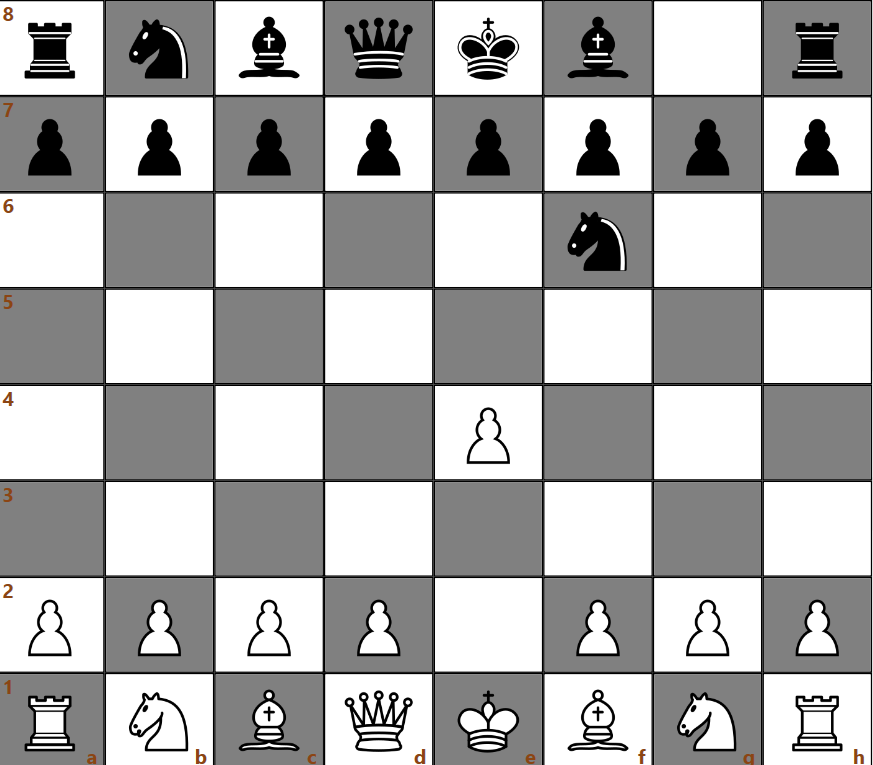
\includegraphics[width=0.6\linewidth]{Images/Test Cases/testCase10Img2.png}
    \caption{After Computer Move}
    \label{fig:AfterComputerMove}
\end{figure}

\section{ER Diagram}

\begin{figure}[H]
    \centering
    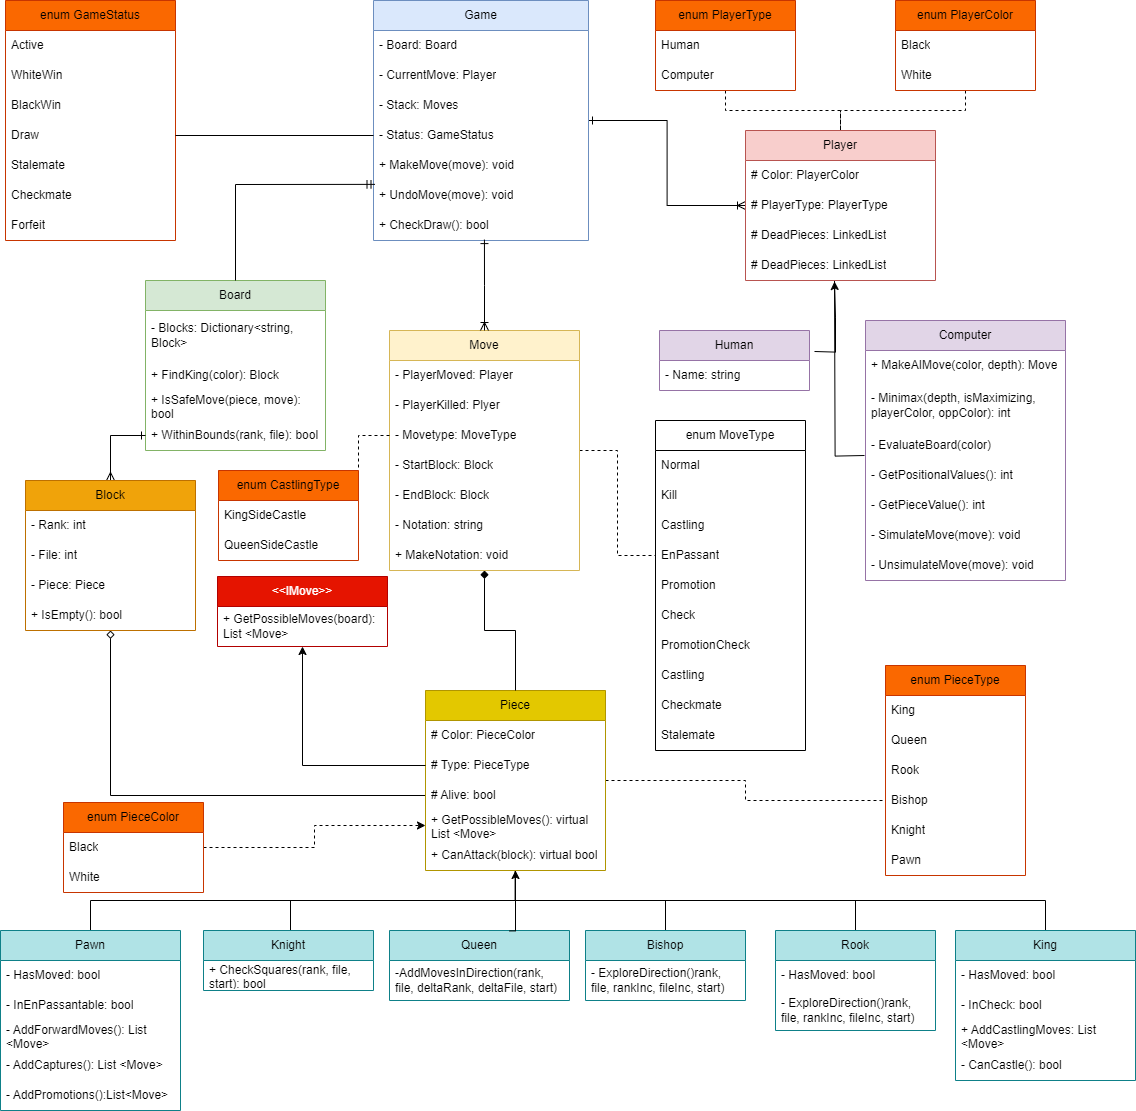
\includegraphics[width=0.7\linewidth]{Images/ERD.png}
    \caption{ER Diagram}
    \label{fig:entityRelationDiagram}
\end{figure}

\section{Implementation}

\subsection{Utility Classes}

The following utility classes provide the functionality required to manage the game's state, players, and pieces:

\begin{itemize}
    \item \textbf{Game}: The Game class orchestrates the entire game flow, including managing the turns, checking for win conditions, and initializing the board. It handles player interactions and keeps track of the game state.
    \item \textbf{Player}: This is the base class for both human and computer players. It defines attributes common to all players and includes methods for making moves and interacting with the board.
    \item \textbf{Board}: The Board class represents the chessboard, holding the blocks and pieces on the board. It is responsible for initializing the board, placing pieces in their starting positions, and updating the board state.
    \item \textbf{Block}: A Block represents an individual square on the chessboard, storing information about the piece occupying the square and its rank and file.
    \item \textbf{Move}: The Move class represents a single move made by a player. It stores the starting and ending positions, along with any special move actions like castling or en passant.
    \item \textbf{Piece}: The base class for all chess pieces. It defines common attributes and movement rules for the pieces, including color, type, and position.
    \item \textbf{King, Pawn, Queen, Bishop, Knight, Rook}: These classes represent specific types of chess pieces, inheriting from the Piece class and implementing their unique movement rules.
    \item \textbf{Human}: The Human class represents a human player, responsible for making moves through user input. It interacts with the game board and manages human-specific gameplay logic.
    \item \textbf{Computer}: The Computer class represents an AI player. It uses algorithms to evaluate moves and make decisions based on the state of the game.
\end{itemize}

\subsection{Data Structures Used}

The data structures utilized in the Chess game are designed to support efficient gameplay, move management, and game state tracking:

\begin{itemize}
    \item \textbf{Array}: Arrays are used for small, fixed-size tasks such as storing specific piece attributes or temporarily holding data during computations.
    \item \textbf{List}: A List is used to store the possible moves for a player. It allows efficient iteration over all possible moves and provides an easy way to manage and evaluate them.
    \item \textbf{LinkedList}: The LinkedList is used to store dead pieces, keeping track of captured pieces. This allows easy modification and retrieval of captured pieces throughout the game.
    \item \textbf{Stack}: The Stack data structure is employed for move management and undo functionality. It stores a history of moves, allowing players to undo actions using the last-in, first-out (LIFO) principle.
    \item \textbf{Adjacency List (Graph)}: The adjacency list represents the connections between blocks on the board as a graph. It treats each block on the screen as node and it's possible moves are edges. It helps efficiently manage the possible movements of pieces by storing neighboring blocks.
\end{itemize}

\subsection{Algorithms Used}

The following algorithms are used to enhance decision-making and evaluate game positions:

\begin{itemize}
    \item \textbf{Minimax}: The Minimax algorithm is a decision-making strategy used by the AI to determine the best possible move by exploring all possible moves and selecting the one that maximizes the AI's chances of winning while minimizing the opponent's advantage.
    \item \textbf{Alpha-Beta Pruning}: Alpha-Beta pruning is an optimization of the Minimax algorithm. It reduces the number of nodes evaluated in the game tree by pruning branches that will not affect the outcome, thus improving performance and making the AI faster.
\end{itemize}

\subsection{Directory Structure}
This figure shows the directories of the project:
\begin{figure}[H]
    \centering
    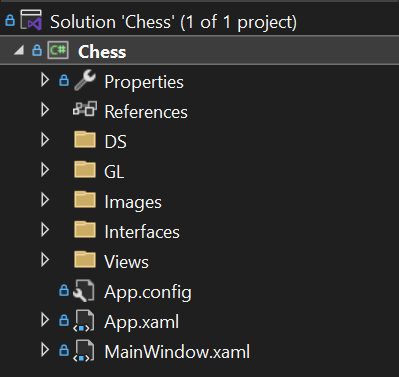
\includegraphics[width=0.5\linewidth]{Images/DirectoryStructure.png}
    \caption{Directory Structure}
    \label{fig:directoryStructure}
\end{figure}

\begin{itemize}
    \item \textbf{DS}: It stores the class files for the data structures that are custom implemented for this project. 
    \item \textbf{GL}: Game Logic (GL) directory stores all the files that are necessary for game logic such as Game.cs, Player.cs, Board.cs, etc. It further contains two subdirectories:
    \begin{itemize}
        \item \textbf{Players}: Stores the implementation for Human and Computer classes.
        \item \textbf{Pieces}: Contains all the pieces such as Pawn, King, Knight, etc.
    \end{itemize}
    \item \textbf{Images}: Contains the images of all the chess pieces.
    \item \textbf{Interface}: Stores the interface IMove.cs that is used in this project to get the possible moves of each piece.
    \item \textbf{Views}: This folder contains all the User Interface files. All of the xaml and xaml.cs code is stored here.
\end{itemize}


\subsection{Code}

\begin{itemize}
    \item \textbf{FindKing(PieceColor pieceColor)}: 
    This function searches for the King piece of the specified color on the board. It iterates through all the blocks and checks if a block contains a piece of type King and the specified color. If found, it returns the block that contains the King.

    \begin{verbatim}
    public Block FindKing(PieceColor pieceColor)
    {
        return Blocks.Values.FirstOrDefault(block =>
        {
            Piece piece = block.GetPiece();
            return piece?.GetPieceType() == PieceType.King && piece.GetColor() == pieceColor;
        });
    }
    \end{verbatim}

    \item \textbf{IsKingInCheck(PieceColor pieceColor)}:
    This function checks if the King of the specified color is in check. It first finds the King using the \texttt{FindKing} method. Then, it checks all blocks on the board to see if any opponent piece can attack the King, considering both pawns and other pieces.

    \begin{verbatim}
    public bool IsKingInCheck(PieceColor pieceColor)
    {
        Block kingBlock = FindKing(pieceColor);
        if (kingBlock == null)
            return false;

        foreach (var block in Blocks.Values)
        {
            Piece attackingPiece = block.GetPiece();
            if (attackingPiece == null || attackingPiece.GetColor() == pieceColor)
                continue;

            if (attackingPiece.GetPieceType() == PieceType.Pawn && attackingPiece.IsAttackingKing(this, kingBlock))
                return true;

            if (attackingPiece.CanAttack(kingBlock, this))
                return true;
        }
        return false;
    }
    \end{verbatim}

    \item \textbf{WithinBounds(int rank, int file)}:
    This function checks if the given rank and file are within the bounds of the chessboard (0 to 7). It returns \texttt{true} if the coordinates are valid, and \texttt{false} otherwise.

    \begin{verbatim}
    public bool WithinBounds(int rank, int file)
    {
        return rank >= 0 && rank < 8 && file >= 0 && file < 8;
    }
    \end{verbatim}

    \item \textbf{AddMovesInDirection(int rank, int file, int deltaRank, int deltaFile, Block startBlock, Board board)}:
    This method adds valid moves in a specified direction to the list of possible moves for a piece. It moves step by step in a given direction (specified by \texttt{deltaRank} and \texttt{deltaFile}) and checks if the destination block is empty or contains an opponent's piece. It stops further movement when an obstacle is encountered.

    \begin{verbatim}
    private void AddMovesInDirection(int rank, int file, int deltaRank, int deltaFile, Block startBlock, Board board)
    {
        for (int i = 1; i < 8; i++)
        {
            int newRank = rank + i * deltaRank;
            int newFile = file + i * deltaFile;

            if (!board.WithinBounds(newRank, newFile))
                break;

            Block endBlock = board.GetBlock(newRank, newFile);

            if (endBlock.IsEmpty() && board.IsSafeMove(this, endBlock))
            {
                possibleMoves.Add(new Move(startBlock, endBlock, this, null));
            }
            else
            {
                if (endBlock?.GetPiece() != null) // stop further movement in this direction
                {
                    if (endBlock.GetPiece().GetColor() != this.GetColor() && board.IsSafeMove(this, endBlock))
                    {
                        possibleMoves.Add(new Move(startBlock, endBlock, this, endBlock.GetPiece()));
                    }
                    break;
                }
                if ((endBlock.GetPiece() != null && endBlock.GetPiece().GetColor() != this.GetColor()) && board.IsSafeMove(this, endBlock))
                {
                    possibleMoves.Add(new Move(startBlock, endBlock, this, endBlock.GetPiece()));
                }
            }
        }
    }
    \end{verbatim}

    \item \textbf{CanAttack(Block targetBlock, Board board)}:
    This method determines if a piece can attack a target block. It checks if the piece can move to the target block either diagonally, horizontally, or vertically. The function returns \texttt{true} if the path is clear, allowing the piece to attack the target block.

    \begin{verbatim}
    public override bool CanAttack(Block targetBlock, Board board)
    {
        Block currentBlock = board.GetBlock(this);
        int rank = currentBlock.GetRank();
        int file = currentBlock.GetFile();

        int targetRank = targetBlock.GetRank();
        int targetFile = targetBlock.GetFile();

        if (Math.Abs(rank - targetRank) == Math.Abs(file - targetFile)) // Diagonal movement
        {
            return board.IsPathClear(rank, file, targetRank, targetFile);
        }
        else if (rank == targetRank || file == targetFile) // Horizontal or vertical movement
        {
            return board.IsPathClear(rank, file, targetRank, targetFile);
        }

        return false;
    }
    \end{verbatim}

    \item \textbf{EnPassant(PieceColor pieceColor, Block currentBlock, int rank, int file, int direction)}: 
    This function checks for the possibility of an en passant capture. It checks if the current rank is the rank where en passant can occur (based on the piece color). If the rank matches, it checks adjacent blocks for opponent pawns that are eligible for en passant and adds possible moves for the current piece to capture them.

    \begin{verbatim}
    public void EnPassant(PieceColor pieceColor, Block currentBlock, int rank, int file, int direction)
    {
        int enPassantRank = (GetColor() == PieceColor.White) ? 3 : 4;

        if (board.GetFirstPlayerColor() == PlayerColor.Black)
            enPassantRank = (GetColor() == PieceColor.White) ? 4 : 3;

        if (rank == enPassantRank)
        {
            foreach (int offset in new[] { -1, 1 })
            {
                if (!board.WithinBounds(rank, file + offset))
                {
                    continue;
                }

                Block sideBlock = board.GetBlock(rank, file + offset);
                if (sideBlock != null && !sideBlock.IsEmpty() &&
                    sideBlock.GetPiece().GetPieceType() == PieceType.Pawn &&
                    ((Pawn)sideBlock.GetPiece()).GetEnPassantable() &&
                    sideBlock.GetPiece().GetColor() != GetColor())
                {
                    Block endBlock = board.GetBlock(rank + direction, file + offset);
                    if (board.IsSafeMove(this, endBlock))
                        moves.Add(new Move(currentBlock, endBlock, this, sideBlock.GetPiece()));
                }
            }
        }
    }
    \end{verbatim}

    \item \textbf{MakeNotation()}: 
    This function generates the algebraic notation for the move made by the piece. It handles different types of moves such as castling, capturing, and promotion. It also takes into account check and checkmate scenarios, appending appropriate symbols to the notation.

    \begin{verbatim}
    public void MakeNotation()
    {
        if (MoveType == MoveType.Draw)
            return;

        if (MoveType == MoveType.Castling && CastlingType == CastlingType.KingSideCastle)
        {
            Notation = "O-O";
            return;
        }
        if (MoveType == MoveType.Castling && CastlingType == CastlingType.QueenSideCastle)
        {
            Notation = "O-O-O";
            return;
        }

        if (PieceMoved.GetPieceType() != PieceType.Pawn)
        {
            Notation = GetPieceMovedString(PieceMoved.GetPieceType());
            // Now we check if any any piece can move to same square
            Piece otherPiece = Board.OtherPieceCanMove(PieceMoved, EndBlock);
            if (otherPiece != null)
            {
                if (Board.GetBlock(otherPiece).GetFile() != StartBlock.GetFile()) // if files are different write just file
                {
                    Notation += GetFileString(StartBlock.GetFile());
                }
                else if (Board.GetBlock(otherPiece).GetFile() == StartBlock.GetFile() // if files are same but ranks are different write just rank
                      && Board.GetBlock(otherPiece).GetRank() != StartBlock.GetRank())
                {
                    Notation += Board.TranslateRank(StartBlock.GetRank());
                }
                else // if both are same write rank and file both
                {
                    Notation += GetFileString(StartBlock.GetFile()) + Board.TranslateRank(StartBlock.GetRank());
                }
            }
            if (PieceKilled == null)
            {
                Notation += GetFileString(EndBlock.GetFile());
            }
        }
        else
        {
            Notation = GetPieceMovedString(PieceMoved.GetPieceType()) + GetFileString(StartBlock.GetFile());
        }

        if (PieceKilled != null)
            Notation += "x" + GetFileString(EndBlock.GetFile());

        Notation += Board.TranslateRank(EndBlock.GetRank());

        if (MoveType == MoveType.Promotion)
            Notation += "=" + GetPieceMovedString(PromotedPieceType);

        if (MoveType == MoveType.Checkmate)
            Notation += "#";
        else if (MoveType == MoveType.Check)
            Notation += "+";

        if (MoveType == MoveType.PromotionCheck)
            Notation += "=" + GetPieceMovedString(PromotedPieceType) + "+";
    }
    \end{verbatim}

    \item \textbf{EvaluateBoard(PlayerColor aiColor)}: 
    This function evaluates the board state from the perspective of the AI's color. It sums up the values of all pieces on the board, factoring in the piece's type and its positional value on the board. The score is positive for the AI's color and negative for the opponent's color.

    \begin{verbatim}
    private int EvaluateBoard(PlayerColor aiColor)
    {
        int score = 0;

        foreach (var block in Board.GetBlocks().Values)
        {
            if (!block.IsEmpty())
            {
                Piece piece = block.GetPiece();
                int pieceValue = GetPieceValue(piece.GetPieceType());
                int positionalBonus = GetPositionalValue(piece, block);

                score += (piece.GetColor().ToString() == aiColor.ToString())
                         ? (pieceValue + positionalBonus)
                         : -(pieceValue + positionalBonus);
            }
        }
        return score;
    }
    \end{verbatim}

    \item \textbf{GetPositionalValue(Piece piece, Block block)}: 
    This function calculates the positional value of a piece based on its location on the board. The value rewards control of the center and provides bonuses for pieces in strategic positions.

    \begin{verbatim}
    private int GetPositionalValue(Piece piece, Block block)
    {
        // Reward control of the center
        int[,] positionalValues = new int[8, 8]
        {
            { 1, 1,  1,  1,  1,  1, 1, 1 },
            { 1, 5,  5,  5,  5,  5, 5, 1 },
            { 1, 5, 10, 10, 10, 10, 5, 1 },
            { 1, 5, 10, 20, 20, 10, 5, 1 },
            { 1, 5, 10, 20, 20, 10, 5, 1 },
            { 1, 5, 10, 10, 10, 10, 5, 1 },
            { 1, 5,  5,  5,  5,  5, 5, 1 },
            { 1, 1,  1,  1,  1,  1, 1, 1 }
        };

        return positionalValues[block.GetRank(), block.GetFile()];
    }
    \end{verbatim}

    \item \textbf{GetPieceValue(PieceType pieceType)}: 
    This function assigns a value to a piece based on its type. The values are commonly used in chess AI for evaluating material advantage.

    \begin{verbatim}
    private int GetPieceValue(PieceType pieceType)
    {
        switch (pieceType)
        {
            case PieceType.Pawn:
                return 1;
            case PieceType.Knight:
                return 3;
            case PieceType.Bishop:
                return 3;
            case PieceType.Rook:
                return 5;
            case PieceType.Queen:
                return 9;
            case PieceType.King:
                return 90;
            default:
                return 0;
        }
    }
    \end{verbatim}
\end{itemize}

\section{Repository Link}
The repository for this project on GitHub: 
\href{https://github.com/mb0227/Chess}{https://github.com/mb0227/Chess}.
\newline
You can also just run the setup file and enjoy the game.
\href{https://github.com/mb0227/Chess/releases/tag/Chess}{Setup}.
It is also available in github repository of this project as a zip file named as Setup.zip. 

\section{Conclusion}

\subsection{Summary}
This Chess Game Project is designed to understand the practical application of data structures in real-world projects. The game was developed using WPF and the .NET Framework, specifically .NETFramework, Version=v4.8. It supports both Multiplayer and Player Vs Computer modes, with three levels of AI difficulty: Easy, Medium, and Hard. The project also features time controls, allowing users to choose between 1-minute, 3-minute, 5-minute, or 10-minute time limits. The game follows the FIDE rules, including specialized moves like En Passant and Castling, and offers Undo functionality along with the ability to draw. 

This project helped me deepen my understanding of implementing data structures, like stacks, linked lists, and graphs, in complex scenarios. It also provided a comprehensive view of how to manage game logic and UI components, and how various design patterns can be applied to create a smooth gaming experience.

\subsection{Challenges Faced}
\begin{itemize}
    \item Developing the game using WPF for the first time, as I had no prior experience with it before.
    \item Working solo on the project, which meant managing all aspects of development by myself.
    \item Debugging special moves like En Passant and Castling, especially when ensuring that the first player could select either White or Black.
    \item Ensuring that the board accurately reflected moves and changes in dead pieces in the UI. This required seamless integration of game logic and the user interface.
    \item Another big challenge was while undoing a move, especially in the moves in which a piece was killed, removing it from the UI was quite a challenge but with a lot of research I overcame it. 
\end{itemize}

\subsection{Project's Weaknesses}
\begin{itemize}
    \item A logical error occurs when trying to manage notations after undoing a move, causing the game to lose track of the correct move notation.
    \item The AI functionality is somewhat weak, as it only evaluates moves based on two factors: positional value and piece value. This limited evaluation results in a less challenging AI opponent.
    \item Introducing additional evaluation conditions causes stack overflow errors, indicating the AI’s evaluation logic needs to be improved.
\end{itemize}

\subsection{Future Enhancements}
\begin{itemize}
    \item Add Redo move functionality, allowing players to redo moves after undoing them.
    \item Implement Pre-Move functionality, enabling players to plan their moves in advance.
    \item Integrate the game with the internet, as it is currently set up locally.
    \item Improve the UI, including displaying move notations simultaneously for both players, instead of after both players have made their moves which is the current implementation.
    \item Enhance the AI by evaluating the board in greater depth, considering more factors for better move determination.
    \item Use of data structures like Trees to do best move analysis.
    \item Implementing Chess 960 which is personally my favourite mode of Chess.
\end{itemize}

\section{Acknowledgments}
I would like to express my sincere gratitude to my instructor Mr. Nazeef-ul-Haq for his dedication in teaching DSA in such a practical way. I would also like to thank my friend Talha Aslam and my senior Muhammad Wali for recommending WPF. I also appreciate the helpful resources and discussions on online forums such as Stack Overflow, which helped me overcome many challenges. Even while writing this documentation, since I am new to LaTeX, I am constantly visiting their website to learn something new. Special thanks to the WPF documentation and the .NET community for providing the necessary tools and insights that made this project possible.

\section{References}
\begin{itemize}
    \item \textbf{WPF Documentation - Microsoft:} \url{https://docs.microsoft.com/en-us/dotnet/desktop/wpf/}.
    \item \textbf{Introduction to AI in Chess - ChessBase:} \url{https://www.chessbase.com/}.
    \item \textbf{C\# Programming Guide - Microsoft:} \url{https://docs.microsoft.com/en-us/dotnet/csharp/programming-guide/}.
    \item \textbf{Chess.com:} \url{https://www.chess.com}. 
    \item \textbf{Lichess}: \url{https://lichess.org}. 
    \item \textbf{GeeksforGeeks}: \url{https://www.geeksforgeeks.org}.
    \item \textbf{FIDE (Fédération Internationale des Échecs)}: \url{https://www.fide.com}.
    \item \textbf{Chess Talk - Chess Notations}: \url{https://www.youtube.com/watch?v=b6PR885Rgb8}. 
    \item \textbf{Kampa Plays - WPF Tutorial}: \url{https://www.youtube.com/watch?v=t9ivUosw_iI&list=PLih2KERbY1HHOOJ2C6FOrVXIwg4AZ-hk1}.
    \item \textbf{Green Chess - Piece Images}:  \url{https://greenchess.net/info.php?item=downloads}. 
\end{itemize}

\end{document}
